\documentclass{beamer}
%
% Choose how your presentation looks.
%
% For more themes, color themes and font themes, see:
% http://deic.uab.es/~iblanes/beamer_gallery/index_by_theme.html
%
\mode<presentation>
{
  \usetheme{Madrid}      % or try Darmstadt, Madrid, Warsaw, ...
  \usecolortheme{beaver} % or try albatross, beaver, crane, ...
  \usefonttheme{serif}  % or try serif, structurebold, ...
  \setbeamertemplate{navigation symbols}{}
  \setbeamertemplate{caption}[numbered]
} 

\usepackage[english]{babel}
\usepackage[utf8x]{inputenc}
\usepackage{multirow}
\usepackage{graphicx}
\usepackage{multicol}
\setlength{\columnseprule}{1pt}
\def\columnseprulecolor{\color{blue}}
\usepackage{color, colortbl}
\usepackage{xcolor}
\usepackage{soul}
\newcommand{\mathcolorbox}[2]{\colorbox{#1}{$\displaystyle #2$}}
\usepackage{amsmath}
\usepackage{mathtools}
\usepackage{extarrows}
\usepackage{listings}
\lstset
{
    language=[LaTeX]TeX,
    breaklines=true,
    basicstyle=\tt\scriptsize,
    %commentstyle=\color{green}
    keywordstyle=\color{blue},
    %stringstyle=\color{black}
    identifierstyle=\color{magenta},
}

\title[Winter School 2020]{Comprehensive Security Analysis of \texttt{CRAFT}}
\author[Hosein Hadipour]{\underline{\textbf{Hosein Hadipour}}\inst{1} \and Sadegh Sadeghi\inst{2} \and Majid M. Niknam\inst{2} \and Nasour Bagheri\inst{4}}
\institute[]{\inst{1} University of Tehran, Iran
\and \inst{2} Kharazmi University, Iran
\and \inst{4} Shahid Rajaee Teacher Training University, Iran}

\date{Feb 2, 2020}
\titlegraphic{
\includegraphics[height=0.1\paperheight]{./Images/logos.pdf}}

\AtBeginSection[]
{
  \begin{frame}<beamer>
    \frametitle{Outline}
    \tableofcontents[currentsection,currentsubsection]
  \end{frame}
}

\begin{document}

\begin{frame}
  \titlepage
\end{frame}


% Uncomment these lines for an automatically generated outline.
\begin{frame}{Outline}
  \tableofcontents
\end{frame}

\section{\texttt{CRAFT} Specifiction}
\begin{frame}{\texttt{CRAFT}\cite{Craft}}
    \begin{itemize}
    \item \texttt{CRAFT}: A light-weight tweakable block cipher, taking efficient protection against DFA\footnote{Differential Fault Attack} in consideration, from design phase
        \item{Main Parameters}: 64-bit block, 128-bit key, 64-bit tweak
        % \item{Internal State}: viewed as a $4\times 4$ array of nibbles
        % \item{Round Function}: \texttt{CRAFT} applies five different operations on the internal state in each round 
    \end{itemize}
\begin{center}
    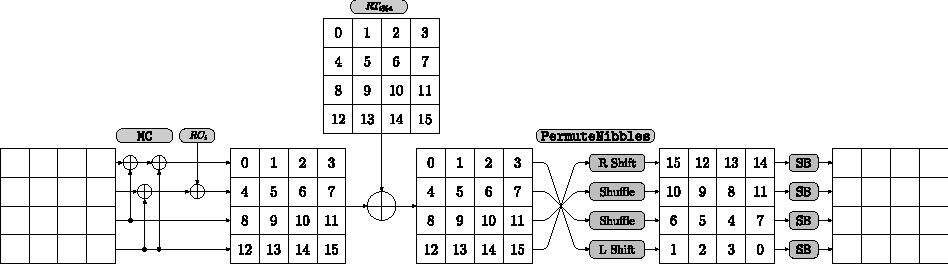
\includegraphics[scale=0.7]{./Images/craft_round_function.pdf}
\end{center}
\end{frame}

\begin{frame}{\texttt{CRAFT}}
\begin{center}
        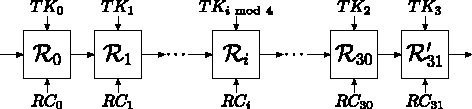
\includegraphics[scale = 0.9 ]{./Images/craft_structure_32r.pdf}
\end{center}
\begin{itemize}
    \item{Structure}: 32 rounds consisting of 31 identical round, plus one linear round (without \texttt{PN}, and \texttt{SB} layers)
    \begin{align*}
    TK_0&=K_0\oplus T,  & TK_1&=K_1\oplus T,\\
    TK_2&=K_0\oplus Q(T),& TK_3&=K_1\oplus Q(T),
    \end{align*}
    
    where $K = K_{0}\|K_{1}\in \mathbb{F}_{2}^{64}\times\mathbb{F}_{2}^{64}$ is the secret key, and $T\in \mathbb{F}_{2}^{64}$ is the master tweak. 
    \item $Q$ is a permutation on the position of tweak nibbles
\end{itemize}
    
\end{frame}
% \begin{frame}{Motivation}
% 	\begin{itemize}
%   		\item Most engineers are lazy ... and that is often a good thing
%   		\begin{itemize}
% 			\item (\textit{lazy} $=$ \textit{to do things in the most efficient way})
% 		\end{itemize}
%   		\pause
%   		\item Engineers are terrible story tellers ... they prefer content to form
%   		\pause
%   		\item Readers are lazy ... need self contained and easy to read material
%   		\pause 
%   		\item \LaTeX{} can help
%   	\end{itemize}
% \end{frame}

% \begin{frame}{Why \LaTeX{} ?}
% 	\begin{itemize}
%   		\item If everyone is lazy, why not use \textit{Word} / \textit{PowerPoint} ?
%   		\pause
%   		\item In \textit{Word} / \textit{PowerPoint} it is easy to make bad things.
%   		\pause
%   		\item In \LaTeX{} it is hard to do bad things.
%   		\pause
%   		\item \LaTeX{} automates structure and format so the author can focus on content.
%   		\pause
%   		\item \LaTeX{} keeps text, sections, figures, etc. globally well spaced using cool optimization algorithms!
%   		\pause
%   		\item \LaTeX{} is better to keep uniform the material contributed by different authors.
% 	\end{itemize}
% \end{frame}

\section{Zero-Correlation Cryptanalysis of \texttt{CRAFT}}
\begin{frame}{Reviewing Some Rules About Linear Masks Propagation}
\begin{center}
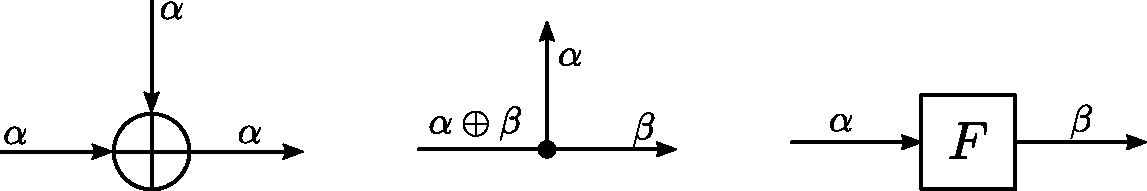
\includegraphics[scale=0.6]{./Images/linear_rules.pdf}
\end{center}
\end{frame}

\begin{frame}{Impact of Considering Tweakey Schedule on ZC Distinguisher}
\begin{itemize}
    \item Consider a toy tweakable block cipher like this:
\end{itemize}
\begin{figure}
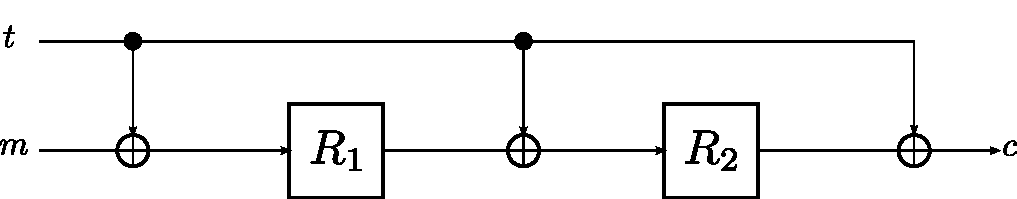
\includegraphics[scale=0.7]{./Images/simple_toy_tbc.pdf}
\centering
\end{figure}
\begin{itemize}
    \item Suppose that the same tweak is used for each round
\end{itemize}
\end{frame}

\begin{frame}{Impact of Considering Tweakey Schedule on ZC Distinguisher}
\begin{itemize}
    \item Remove the tweakey schedule, and propagate the linear masks through the data path
\end{itemize}
\begin{figure}
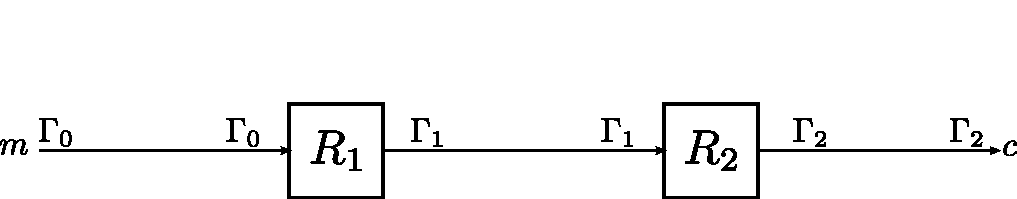
\includegraphics[scale=0.7]{./Images/impact_of_tk_1.pdf}
\centering
\end{figure}
\end{frame}

\begin{frame}{Impact of Considering Tweakey Schedule on ZC Distinguisher}
\begin{itemize}
    \item Now, Consider the tweakey schedule in the analysis. What will be happened for the previous propagation?
\end{itemize}
\begin{figure}
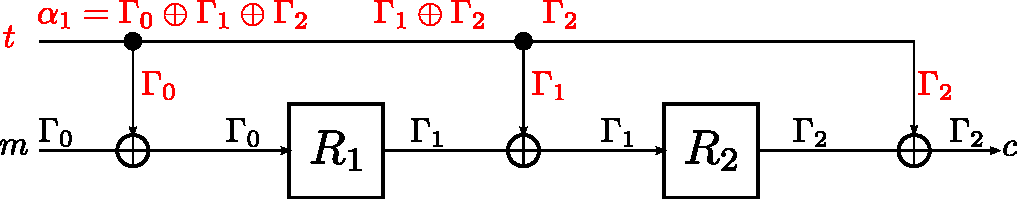
\includegraphics[scale=0.7]{./Images/impact_of_tk_2.pdf}
\centering
\end{figure}
\end{frame}

\begin{frame}{Impact of Considering Tweakey Schedule on ZC Distinguisher}
\begin{figure}
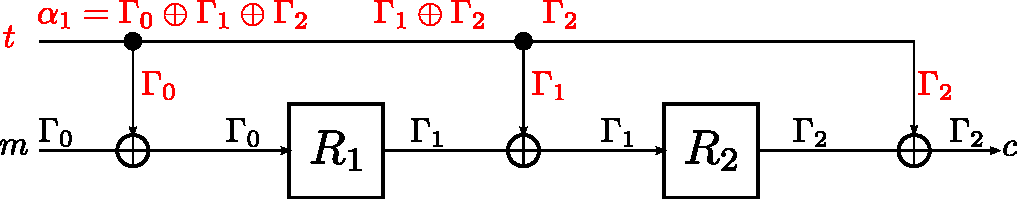
\includegraphics[scale=0.7]{./Images/impact_of_tk_2.pdf}
\centering
\end{figure}
\begin{itemize}
    \item No extra linear trail will be crated
    \item The following extra restriction is induced by the tweakey schedule: 
    \[
    \textcolor{red}{\alpha_{1} = \Gamma_{0} \oplus \Gamma_{1}\oplus \Gamma_{2}}
    \]
    \item The extra constraint, increases the probability of existing a zero-correlation linear hull \cite{Tweakable-Zero-Correlation}
\end{itemize}
\end{frame}
% \subsection{Improving the Zero-Correlation Distingusiher of \texttt{CRAFT}}

% % \begin{frame}{Single Tweak Zero-Correlation Distinguisher}
% % \begin{center}
% %     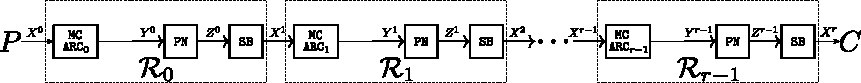
\includegraphics[scale=0.8]{./Images/zc_st_effective_parts.pdf}
% % \end{center}
% % \begin{itemize}
% %     \item $E_{K}(P, T)$: $r$ rounds of \texttt{CRAFT}, where $K$, and $T$ are fixed
% %     \item Correlation of a linear approximation with input/output linear masks $(\alpha, \beta) \in \mathbb{F}_{2}^{64}\times \mathbb{F}_{2}^{64}:$
% %     \[
% %     corr(\alpha, \beta) = 2 \Pr\left( \langle \alpha, P \rangle \oplus \langle \beta, E_{K}(P, T)\rangle  = 0 \right) - 1.
% %     \]
% %     \item Calculation of the correlation, when $\Gamma X^{i}$, and $\Gamma X^{i + 1}$, are the input, and output linear masks of $i + 1$'th round respectively:
% %     \[
% %     corr(\alpha, \beta) = \sum_{\substack{\Gamma X^{0} = \alpha, \Gamma X^{r} = \beta,\\ (\Gamma X^{1}, \cdots , \Gamma X^{r-1})\in (\mathbb{F}_{2}^{64})^{r-1}}} C_{\Gamma},
% %     \], 
% %     where $
% %     C_{\Gamma} = \prod_{i = 0}^{r - 1} corr(\Gamma X^{i},\Gamma X^{i+1})$
% % \end{itemize}
% % \end{frame}

% \begin{frame}{Correlation of a Linear Approximation for a Tweakable Block Cipher}
% \begin{center}
%     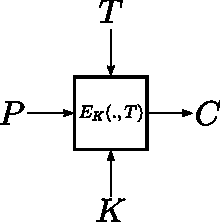
\includegraphics[scale=0.8]{./Images/tweakable_bc.pdf}
% \end{center}
% \begin{itemize}
%     \item Tweak is public parameter, and can be involved in the ZC analysis
%     \item Input linear mask consists of two components, $\alpha_{1}$ for plaintext, and $\alpha_{2}$ for master tweak
%     \item Correlation of a linear approximation with input mask $(\alpha_{1}, \alpha_{2})\in \mathbb{F}_{2}^{n}\times \mathbb{F}_{2}^{t}$, and output mask $\beta \in \mathbb{F}_{2}^{n}$:
%     %  \scalebox{1}{\parbox{.8\linewidth}{
%     \[
%     corr((\alpha_{1}, \alpha_{2}), \beta) = 2 \Pr\left( \langle \alpha_{1}, P \rangle \oplus \langle \alpha_{2}, T \rangle \oplus \langle \beta, E_{K}(P, T)\rangle  = 0 \right) - 1.
%     \]
%     % }}
% \end{itemize}
% \end{frame}

% % \begin{frame}{Impact of Considering Tweakey Schedule in ZC}
% % \begin{center}
% %     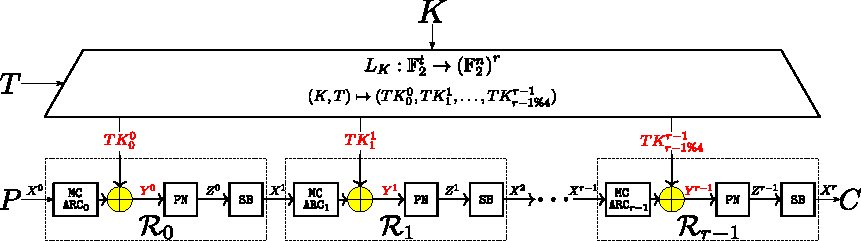
\includegraphics[scale=0.8]{./Images/zc_rt_effective_parts.pdf}
% % \end{center}
% % \begin{itemize}
% %     \item According to the linear tweakey schedule of \texttt{CRAFT}:
% %     \[
% %     \label{relation_between_subtk_masks}
% %     \alpha_{2} = \mathcal{L}(\Gamma Y^{0}, \ldots, \Gamma Y^{r - 1}):= \bigoplus_{\substack{i = 0,\\ i \% 4 < 2}}^{r - 1} \Gamma Y^{i} \oplus \bigoplus_{\substack{i = 0,\\ i \% 4 \geq 2}}^{r - 1} Q^{-1}\left(\Gamma Y^{i}\right),
% %     \]
% %     \item According to the propagation rule of linear masks for \texttt{XOR}:
% %     \[
% %     \Gamma TK_{i \% 4}^{i} = \Gamma Y^{i} , 0 \leq i \leq r  - 1
% %     \]
% % \end{itemize}
% % \end{frame}

% \begin{frame}{Impact of Considering Tweakey Schedule in ZC}
% \begin{center}
%     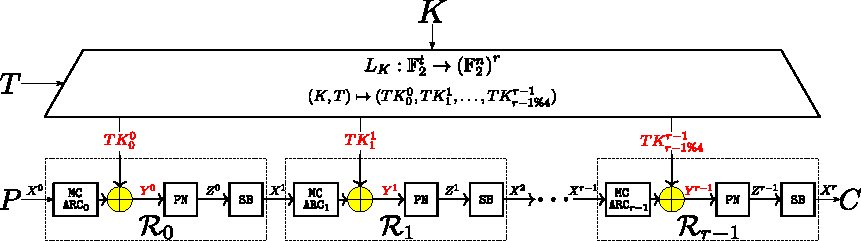
\includegraphics[scale=0.8]{./Images/zc_rt_effective_parts.pdf}
% \end{center}
% % \begin{itemize}
%     % \item The correlation,  when $(\Gamma X^{i}, \Gamma TK_{i\%4}^{i})$, and $\Gamma X^{i + 1}$, are the input, and output linear masks of $i + 1$'th round respectively:
%     \[
%     corr((\alpha_{1}, \alpha_{2}), \beta) = \sum_{\substack{\Gamma X^{0} = \alpha_{1}, \Gamma X^{r} = \beta,\\ (\Gamma X^{1}, \cdots , \Gamma X^{r-1}) \in (\mathbb{F}_{2}^{64})^{r-1}\\\textcolor{red}{\alpha_{2} = \mathcal{L}(\Gamma Y^{0}, \ldots, \Gamma Y^{r - 1})}}} C_{\Gamma}.
%     \]
%     % where
%     \[C_{\Gamma} = \prod_{i = 0}^{r - 1} corr((\Gamma X^{i},\Gamma Y^{i}),\Gamma X^{i+1})\]
% % \end{itemize}
% \end{frame}

% \begin{frame}{Impact of Considering Tweakey Schedule in ZC}
% \begin{center}
%     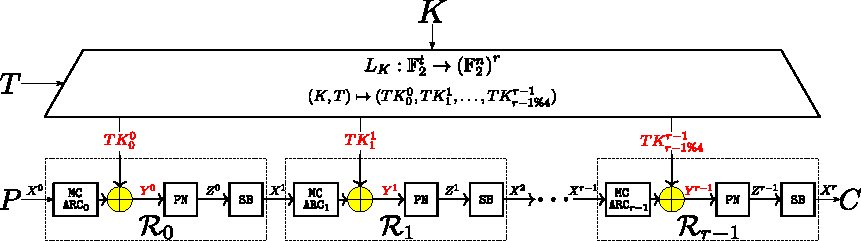
\includegraphics[scale=0.8]{./Images/zc_rt_effective_parts.pdf}
% \end{center}
% \begin{itemize}
%     \item The additional constraint $\alpha_{2} = \mathcal{L}(\Gamma Y^{0}, \ldots, \Gamma Y^{r - 1})$, introduces additional restriction on linear trails that are included in a linear hull
%     \item Additional restriction causes the probability of existing a longer ZC distinguisher to increase \cite{Tweakable-Zero-Correlation}
% \end{itemize}
% \end{frame}

% \begin{frame}{Our strategy to find new ZC distinguishers for \texttt{CRAFT}}
% \begin{fact}
% Linear behaviour of \texttt{CRAFT} depends on the starting round ($RT_{0}, RT_{1}, RT_{2}, RT_{3}$)
% \end{fact}

% \begin{enumerate}
% \item Tasks performed by computer
%     \begin{itemize}
%     \item For each of the cases $RT_{0}, RT_{1}, RT_{2}$, and $RT_{3}$, the problem of finding a valid linear trail covering the given number of rounds, is converted to an MILP problem 
%     \begin{itemize}
%     \item The input, and output linear masks, are fixed to be a binary vector with hamming weight of one ($64\times 64\times 64 = 262144$ possibilities)
%     \item If the obtained MILP problem, for a given fixed input/output masks, becomes infeasible, there is a zero-correlation linear hull with the given input/output masks
%     \end{itemize}
%     \end{itemize}
% \item Task performed by human
%     \begin{itemize}
%         \item The obtained zero-correlation linear hulls, are mathematically proven
%     \end{itemize}
% \end{enumerate}
% \end{frame}

\begin{frame}{Our Strategy to Find New ZC Distinguisher for \texttt{CRAFT}}
\begin{fact}
Linear behaviour of \texttt{CRAFT} depends on the starting round ($RT_{0}, RT_{1}, RT_{2}, RT_{3}$)
\end{fact}
\begin{block}{Tasks Performed by Computer}
% \begin{itemize}
    % \item The problem of finding a valid linear trail, is converted to an MILP problem for each of the cases $RT_{0}, ..., RT_{3}$ separately
    % \item The variables corresponding to the input/output masks are fixed to be a binary vector with hamming weight of one ($64\times 64\times 64 = 262144$ possibilities)
    % \item If the obtained MILP problem, becomes infeasible, the correlation of linear hull with the chosen input/output masks is zero
zero correlation linear hulls are obtained automatically via MILP based method
% \end{itemize}
\end{block}
\begin{block}{Task Performed by Human}
The obtained zero-correlation linear hulls, are mathematically proven
\end{block}
\end{frame}
\subsection{Improving Zero-Correlation Distinguisher of \texttt{CRAFT}}
\begin{frame}{New ZC Distinguishers Covering 14 rounds of \texttt{CRAFT}}
\begin{block}{RT0}
\[\texttt{0000~$\gamma$000~0000~$\gamma$000} \xrightarrow{\text{14-round-$RT_0$}} \texttt{0000~$\delta$000~0000~0000},\]
\[\Gamma T = \texttt{****~****~***8~****}\]
\end{block}

\begin{block}{RT2, and RT3}
\[\texttt{0000~$\gamma$000~0000~0000} \xrightarrow{\text{14-round-$RT_2$}} \texttt{0000~0$\delta$00~0000~0000},\]
\[\texttt{0000~0$\gamma$00~0000~0000} \xrightarrow{\text{14-round-$RT_3$}} \texttt{0000~$\delta$000~0000~0000},\]
\[\Gamma T= \texttt{****~****~***0~****}\]
\end{block}
\begin{itemize}
    \item $\texttt{*}$ depicts an arbitrary value in $\mathbb{F}_{2}^{4}$, and $\gamma, \delta\in \mathbb{F}_{2}^{4}\setminus \{0\}$
    \item We have not found a ZC distinguisher covering 14 rounds, in case $RT_{1}$
\end{itemize}
\end{frame}

\begin{frame}{Proof of 14-round ZC disntinguisher in case $RT0$}
% \begin{columns}
% \column{0.5\textwidth}
% \begin{block}{Forward trail}
% \begin{center}
%     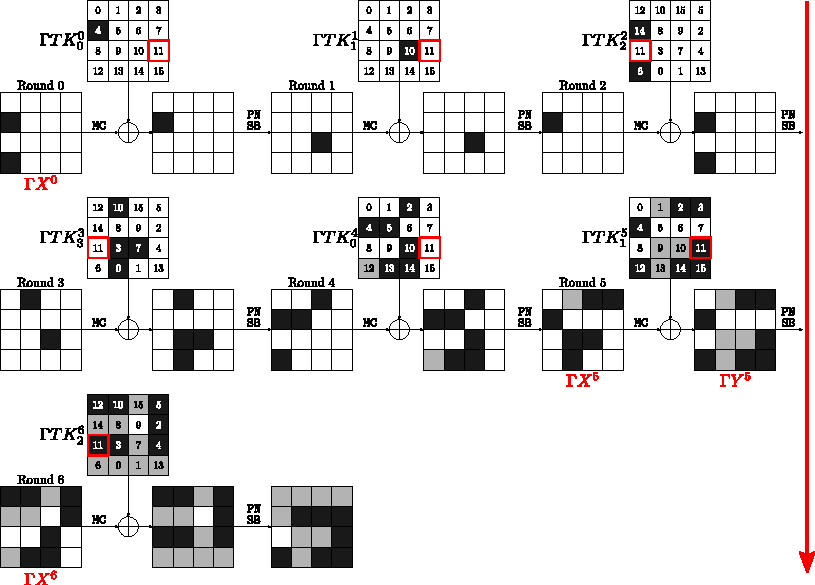
\includegraphics[width=6cm]{./Images/zc_14r_rt0_forward.pdf}
% \end{center}
% \end{block}

% \column{0.5\textwidth}
% \begin{block}{Backward trail}
% \begin{center}
%     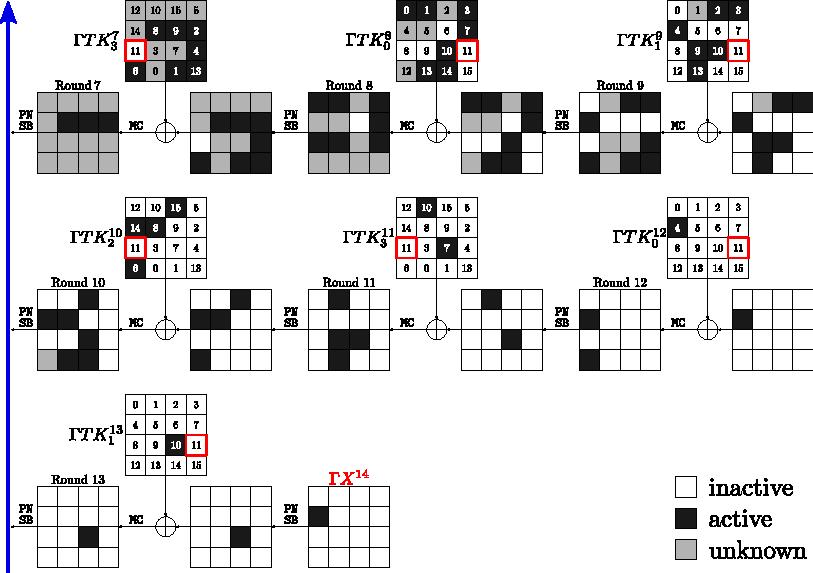
\includegraphics[width=6cm]{./Images/zc_14r_rt0_backward.pdf}
% \end{center}
% \end{block}
% \end{columns}

\begin{center}
    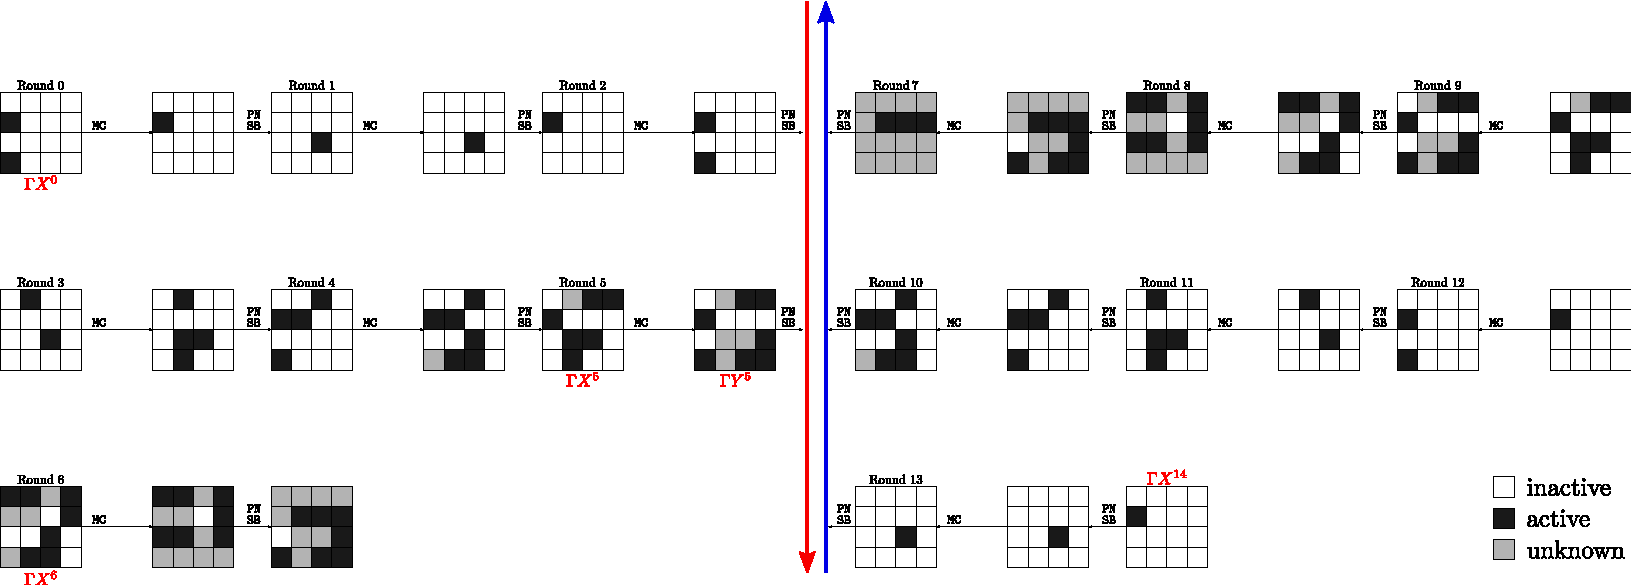
\includegraphics[width = 12cm]{./Images/zc_14r_tk0_0.pdf}
\end{center}
% According to the chosen mask for master tweak, and the linear tweakey schedule:
% \[\Gamma T = \bigoplus_{\substack{i = 0,\\ i \% 4 < 2}}^{r - 1} \Gamma Y_{i} \oplus \bigoplus_{\substack{i = 0,\\ i \% 4 \geq 2}}^{r - 1} Q^{-1}\left( \Gamma Y_{i}\right) = \left( {\begin{array}{*{20}{c}}
% *&*&*&*\\
% *&*&*&*\\
% *&*&*&\texttt{8}\\
% *&*&*&*
% \end{array}} \right)\]
\vspace{1.45cm}
\begin{center}
    What if we consider the tweakey schedule?
\end{center}
\end{frame}

\begin{frame}{Proof of 14-round ZC disntinguisher in case $RT0$}
\begin{center}
    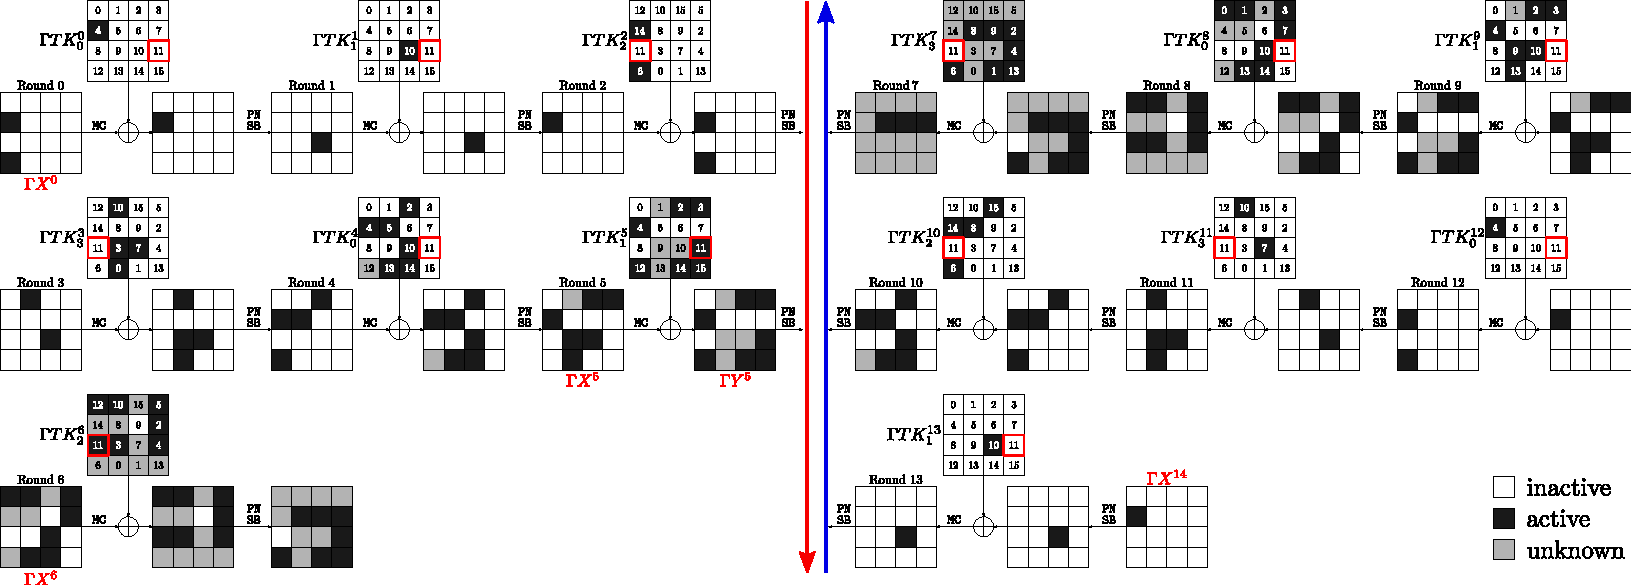
\includegraphics[width = 12cm]{./Images/zc_14r_tk0_1.pdf}
\end{center}
\[\Gamma T = \bigoplus_{\substack{i = 0,\\ i \% 4 < 2}}^{r - 1} \Gamma Y_{i} \oplus \bigoplus_{\substack{i = 0,\\ i \% 4 \geq 2}}^{r - 1} Q^{-1}\left( \Gamma Y_{i}\right) = \left( {\begin{array}{*{20}{c}}
*&*&*&*\\
*&*&*&*\\
*&*&*&\textcolor{red}{\texttt{8}}\\
*&*&*&*
\end{array}} \right)\]
\end{frame}

\begin{frame}{Proof of 14-round ZC disntinguisher in case $RT0$}
\begin{center}
    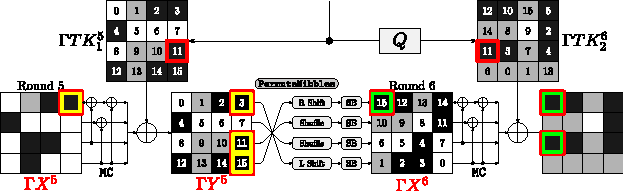
\includegraphics[height = 2.8cm]{./Images/zc_14r_rt0_contradiction_part.pdf}
\end{center}
\begin{block}{According to the tweakey schedule, and \texttt{MC} in rounds 5, and 6}
\[\Gamma TK_{1}^{5}[11] \oplus \Gamma TK_{2}^{6}[8]=\texttt{8}
\xLongrightarrow[\scriptstyle{\Gamma Y^{5}[11] = \Gamma TK_{1}^{5}[11]}]{\scriptstyle{\Gamma X^{6}[0] = \Gamma TK_{2}^{6}[8]}}
\mathcolorbox{yellow}{\Gamma Y^{5}[11]} \oplus \mathcolorbox{green}{\Gamma X^{6}[0]} = \texttt{8}\]
\end{block}

\begin{block}{According to the \texttt{MC}, \texttt{PN}, and \texttt{SB} in round 5}
\[\Gamma Y^{5}[11] = \Gamma Y^{5}[15] \Rightarrow
\mathcolorbox{green}{\Gamma X^{6}[0]} \in LAT[\mathcolorbox{yellow}{\Gamma Y^{5}[11]}]\]
\end{block}
\textcolor{red}{Contradiction}:
$\exists ~ (x, y)\in \mathbb{F}_{2}^{4}\times \mathbb{F}_{2}^4 ~ s.t. ~  (\texttt{LAT}[\colorbox{yellow}{x}][\colorbox{green}{y}] \neq 0) \wedge (\colorbox{yellow}{x} \oplus \colorbox{green}{y} = \texttt{8})$
\end{frame}

\section{Integral Cryptanalysis of \texttt{CRAFT}}
\begin{frame}{Link Between Zero-Correlation and Integral Distinguishers}
\begin{theorem}
\label{linking_zc_to_integral}
\cite{linkZCtoIntergal} Let $F:\mathbb{F}_{2}^{n}\rightarrow \mathbb{F}_{2}^{n}$ be a function, and $A$ be a subspace of $\mathbb{F}_{2}^{n}$ and $\beta\in \mathbb{F}_{2}^{n} \setminus \{0\}$. Suppose that $(\alpha, \beta)$ is a zero-correlation linear approximation for any $\alpha \in A$, then for any $\lambda \in \mathbb{F}_{2}^{n}$, $\langle \beta, F(x + \lambda) \rangle$ is balanced on the following set 
\begin{equation*}
    A^{\bot} = \{x\in \mathbb{F}_{2}^{n} | \langle \alpha, x \rangle = 0, \alpha \in A\}.
\end{equation*}
\end{theorem}
\begin{theorem}
\label{link_nontrivial_zc_to_integral}
\cite{linkZCtoIntergal} A nontrivial zero-correlation linear hull of a block cipher always implies the existence of an integral distinguisher.
\end{theorem}
\end{frame}

\subsection{Improving Integral Distinguishers of \texttt{CRAFT}}

\begin{frame}{New Integral Distinguishers for \texttt{CRAFT}}
\begin{itemize}
    \item Only one nibble of tweak is involved in our ZC distnguishers
    \item Attacker can choose an arbitrary fixed value for those tweak nibbles are not involved in the distinguisher
    \item The domain space of the corresponding integral distinguishers is 68, instead of 128
    \item The required data for the corresponding integral distinguishers must be taken form $A^{\bot}$
    \item The data complexity of the corresponding integral distinguisher eqauls to $2^{\dim(A^{\bot})} = 2^{68 - \dim(A)}$
\end{itemize}
\begin{center}
\begin{tabular}{|c||c|c|c|c|}
\hline
Case & $\dim(A)$ & $\dim(A^{\bot})$ & data complexity & $\sharp$ rounds\\
\hline
$RT_{0}$ & $1$ & $67$ & $2^{67} = 2^{4}\times 2^{63}$ & $14$\\
\hline 
$RT_{2}$ & $4$ & $64$ & $2^{64} = 2^{4}\times 2^{60}$ & $14$\\
\hline
$RT_{3}$ & $4$ & $64$ & $2^{64} = 2^{4}\times 2^{60}$ & $14$\\
\hline
\end{tabular}
\end{center}
\end{frame}

\section{Differential Cryptanalysis of \texttt{CRAFT}}

\begin{frame}{Our Strategy to Evaluate the Differential Effect}
We use \texttt{CryptoSMT}\cite{CryptoSMT-ref} to estimate the differential effect, and it uses the following strategy to enumerate the differential trails in a differential effect \cite{liu2016automatic,kolbl2015observations}:
\vspace{5mm}
\begin{enumerate}
    \item Build the \texttt{CNF} modeling the problem, ask the solver to give one solution $x$ if it exists
    \vspace{3mm}
    \item Add a new condition to the current \texttt{CNF} model in order to remove $x$
    \vspace{3mm}
    \item Ask the solver to give a solution, repeat step 2 until solver returns unsatisfiable
\end{enumerate}

% \texttt{CryptoSMT} uses \texttt{CryptoMiniSat} which supports parallel \texttt{SAT} solving, to evaluate the differential effect
% \vspace{5mm}
% \textcolor{red}{Doesn't matter what solver you use, every solver that uses this strategy, is memory intensive, if the problem has a huge number of solutions}
\end{frame}

% \begin{frame}{First Observations and Motivation}
% \begin{itemize}
%     \item Observations showed that the clustering effect has a great impact on the probability of the differentials:
% \end{itemize}
% \begin{center}
% \scalebox{0.9}{
% \begin{tabular}{c|ccccccc}
% $\sharp$ rounds &1&2&3&4&5&6&7\\\hline
% $\sharp$ Active Sboxes &1&2&4&6&10&14&20\\\hline
%  $-\log_2(DP) \leq $&2&4&8&12&20&28&40\\\hline
% \rowcolor{yellow}
% $-\log_{2}(DP)\leq $&2&2&5&7.04&12.29&16.97&24.96\\\hline
% \end{tabular}}
% \end{center}
% \begin{itemize}
%     \item The results were very promising, but finding even one valid differential trail for large number of rounds is a time consuming job using bit-oriented SAT or MILP models
%     \item We were motivted to find a more efficient way to approximate the differential effect of \texttt{CRAFT} for large number of rounds
% \end{itemize}

% \end{frame}

\subsection{Making the \texttt{CryptoSMT} Faster}
\begin{frame}{Improving the Sbox-Encoding in \texttt{CryptoSMT}}
In order to make the \texttt{CryptoSMT} faster, the following method is used:
    \begin{itemize}
        \item Let $x, y\in \mathbb{F}_{2}^{4}$ are the input/output differences of the Sbox, and $p = (p_{0}, p_{1}, p_{2})$ is used to encode $\Pr\{x\to y\} = 2^{-wt(p)}$
        \item The truth table of the following $11$-bit Boolean function \cite{sun2018more}, is generated at first:
    \end{itemize}
    \begin{center}
    \scalebox{0.7}{\parbox{.8\linewidth}{
    \[
    \begin{array}{ll}
    f(x, y, p) = 0 & if\  \Pr\{x\to y\} = 0,\\
    f(x, y, p) =  
    \begin{cases}
          1 & p = (1, 1, 1)\\
          0 & o.w
    \end{cases} & if\  \Pr\{x\to y\} = 2^{-3},\\
    f(x, y, p) =  
    \begin{cases}
          1 & p = (0, 1, 1)\\
          0 & o.w
    \end{cases} & if\  \Pr\{x\to y\} = 2^{-2},\\
    f(x, y, p) =  
    \begin{cases}
          1 & p = (0, 0, 0)\\
          0 & o.w
    \end{cases} & if\  \Pr\{x\to y\} = 1\\
    \end{array}
    \]
    }}
    \end{center}
    \begin{itemize}
        \item The minimized product-of-sum (CNF) representation of the above Boolean function, is used to model the differential behaviour of Sbox
        % \item The minimized CNF representation can be obtained via Quine-McCluskey\cite{quine1952problem, quine1955way, mccluskey1956minimization}, and Espresso algorithm \cite{brayton1984logic} implemented at the off-the-shelf program Logic Friday\cite{logicfriday_program}
    \end{itemize}
\end{frame}

% % \begin{frame}{\texttt{CryptoSMT} Before and After Optimization}
% % The impact of the optimization on the performance of \texttt{CryptoSMT} through the search for the best single differential characteristic of $r$ rounds of \texttt{CRAFT} in the single tweak model
% % \begin{center}
% % \begin{tabular}{|c|c|c|c|c|c|c|}\hline
% % %\cline{4-7}
% % \multirow{2}{*}{$r$} & \multirow{2}{*}{SW} &\multirow{2}{*}{MW}& \multicolumn{2}{l|}{\cellcolor{green}Optimized} & \multicolumn{2}{l|}{\cellcolor{red}Unoptimized} \\ \cline{4-7}
% % && & STP & Boolector & STP & Boolector\\\hline
% % 1&0&2($2^{-2}$)&\cellcolor{green}0.36 s &0.52 s & \cellcolor{red}34.2 s & 13.53 s \\\hline
% % 2 &2&4($2^{-4}$)&\cellcolor{green} 0.80 s & 1.07 s &\cellcolor{red} 75.07 s &29.69 s\\\hline
% % 3 &4&8($2^{-8}$)&\cellcolor{green} 2.25 s & 2.79 s & \cellcolor{red}195.67 s & 74.78 s\\\hline
% % 4 &8&12($2^{-12}$)&\cellcolor{green} 3.25 s & 4.18 s & \cellcolor{red}313.44 s & 100.83 s\\\hline
% % 5 &12& 20($2^{-20}$) & \cellcolor{green}10.84 s & 13.92 s & \cellcolor{red}831.86 s & 234.95 s\\\hline
% % 6 &20&28($2^{-28}$)& \cellcolor{green}20.55 s & 20.14 s & \cellcolor{red}1249.29 s & 296.06 s\\\hline
% % 7 & 28 & 40($2^{-40}$) & \cellcolor{green}69.03 s & 58.7 s & \cellcolor{red}2703.25 s & 512.25 s\\\hline
% % 8 & 40 &52($2^{-52}$)& \cellcolor{green}179.63 s & 100.07 s & \cellcolor{red}5526.63 s & 664.21 s\\\hline
% % 9 & 52 &64($2^{-64}$)& \cellcolor{green}501.68 s & 190.35 s & \cellcolor{red}9739.49 s & 831.22 s\\\hline
% % \end{tabular}
% % \end{center}
% % \tiny{Computing system's configurations: Intel(R) Core(TM) i5-6600K CPU @ 3.50GHz, 8 Gig RAM, running Ubuntu 18.04 LTS}
% % \end{frame}

% % \begin{frame}{Using Word-Oriented, and Then Bit-Oriented Model}
% % We use the following steps to find an optimum differential trail for the large number of rounds:
% % \begin{enumerate}
% %     \item Using a word-oriented MILP model, find a truncated differential pattern with the minimum number of active S-boxes
% %     \item Based on the found trail from the word-oriented model, develop the constraints for \texttt{CryptoSMT}, to limit the search to the truncated pattern, in the bit-oriented model
% % \end{enumerate}
% % \begin{block}{Result}
% % We were able to find a valid optimum differential trail for large number of rounds very faster than before
% % \end{block}
% % \end{frame}

\begin{frame}{A Light of Hope and A New Issue!}
First Success:
\begin{itemize}
\item 
We found an optimum differetial trail covering 10 rounds of \texttt{CRAFT} with the following input/output differences
\end{itemize}
\begin{center}
\scalebox{0.7}{\parbox{1\linewidth}{
\[\texttt{0AAA~00AA~0000~00AA} \xrightarrow{\text{10-round; ~~$\Pr\geq2^{-50.2554}$}} \texttt{0A00~0000~0000~00AA}\]
}}
\end{center}
\begin{itemize}
\item The input/output differences were fixed, and the optimized \texttt{CryptoSMT} was used to evaluate the differential effect
\item 
3513898 optimal trails were counted in 4 days, before interrupting the run!
\item We could improve the designers' claim ($2^{-62.61}$) at this stage 
\end{itemize}
A new issue:
\begin{itemize}
\item The evaluation of differential effect was still very time consuming! Especially for more number of rounds
\end{itemize}
\end{frame}

% % \begin{frame}{Some Inspiring Observations}
% % \begin{itemize}
% %     \item We observed that the optimum truncated pattern for any input/output differences with the optimum trail that we have checked, are unique!  
% %     \item In order to verify the uniqueness, for a given input/output differences for which there is an optimum trail, we forced the MILP  tools to find an optimum trail with different truncated pattern
% %     \item For all input/output differences that we checked, the programs returned infeasible, which means there is not another truncated pattern
% % \end{itemize}
% % \end{frame}

\begin{frame}{Some Inspiring Observations}
\begin{itemize}
\item We observed that there are optimum trails for even (strating from 8), and odd (starting from 9) number of roudns, with the same input/output differences: 
\end{itemize}
\begin{center}
\scalebox{0.8}{\parbox{1\linewidth}{
\[\texttt{0AAA~00AA~0000~00AA} \xrightarrow{\text{r-round; even, ~~$\Pr^{o,r}_c=2^{-(56+8(r-8))}$}} \texttt{0A00~0000~0000~00AA},\]
}}
\scalebox{0.8}{\parbox{1\linewidth}{
\[\texttt{AA0A~AA00~0000~AA00} \xrightarrow{\text{r-round; odd, ~~$\Pr^{o,r}_c=2^{-(64+8(r-9))}$}}\texttt{0A00~0000~0000~00AA},\] 
}}
\end{center}
\begin{itemize}
\item The above observations, lead us to divide and conquer strategy
\end{itemize}
\end{frame}

\subsection{Divide and Conquer Strategy}
\begin{frame}{Building Blocks of Even Number of Rounds}
% \begin{center}
% \scalebox{0.6}{
% \begin{tabular}{c}
% % Requires \usepackage{graphicx}
% 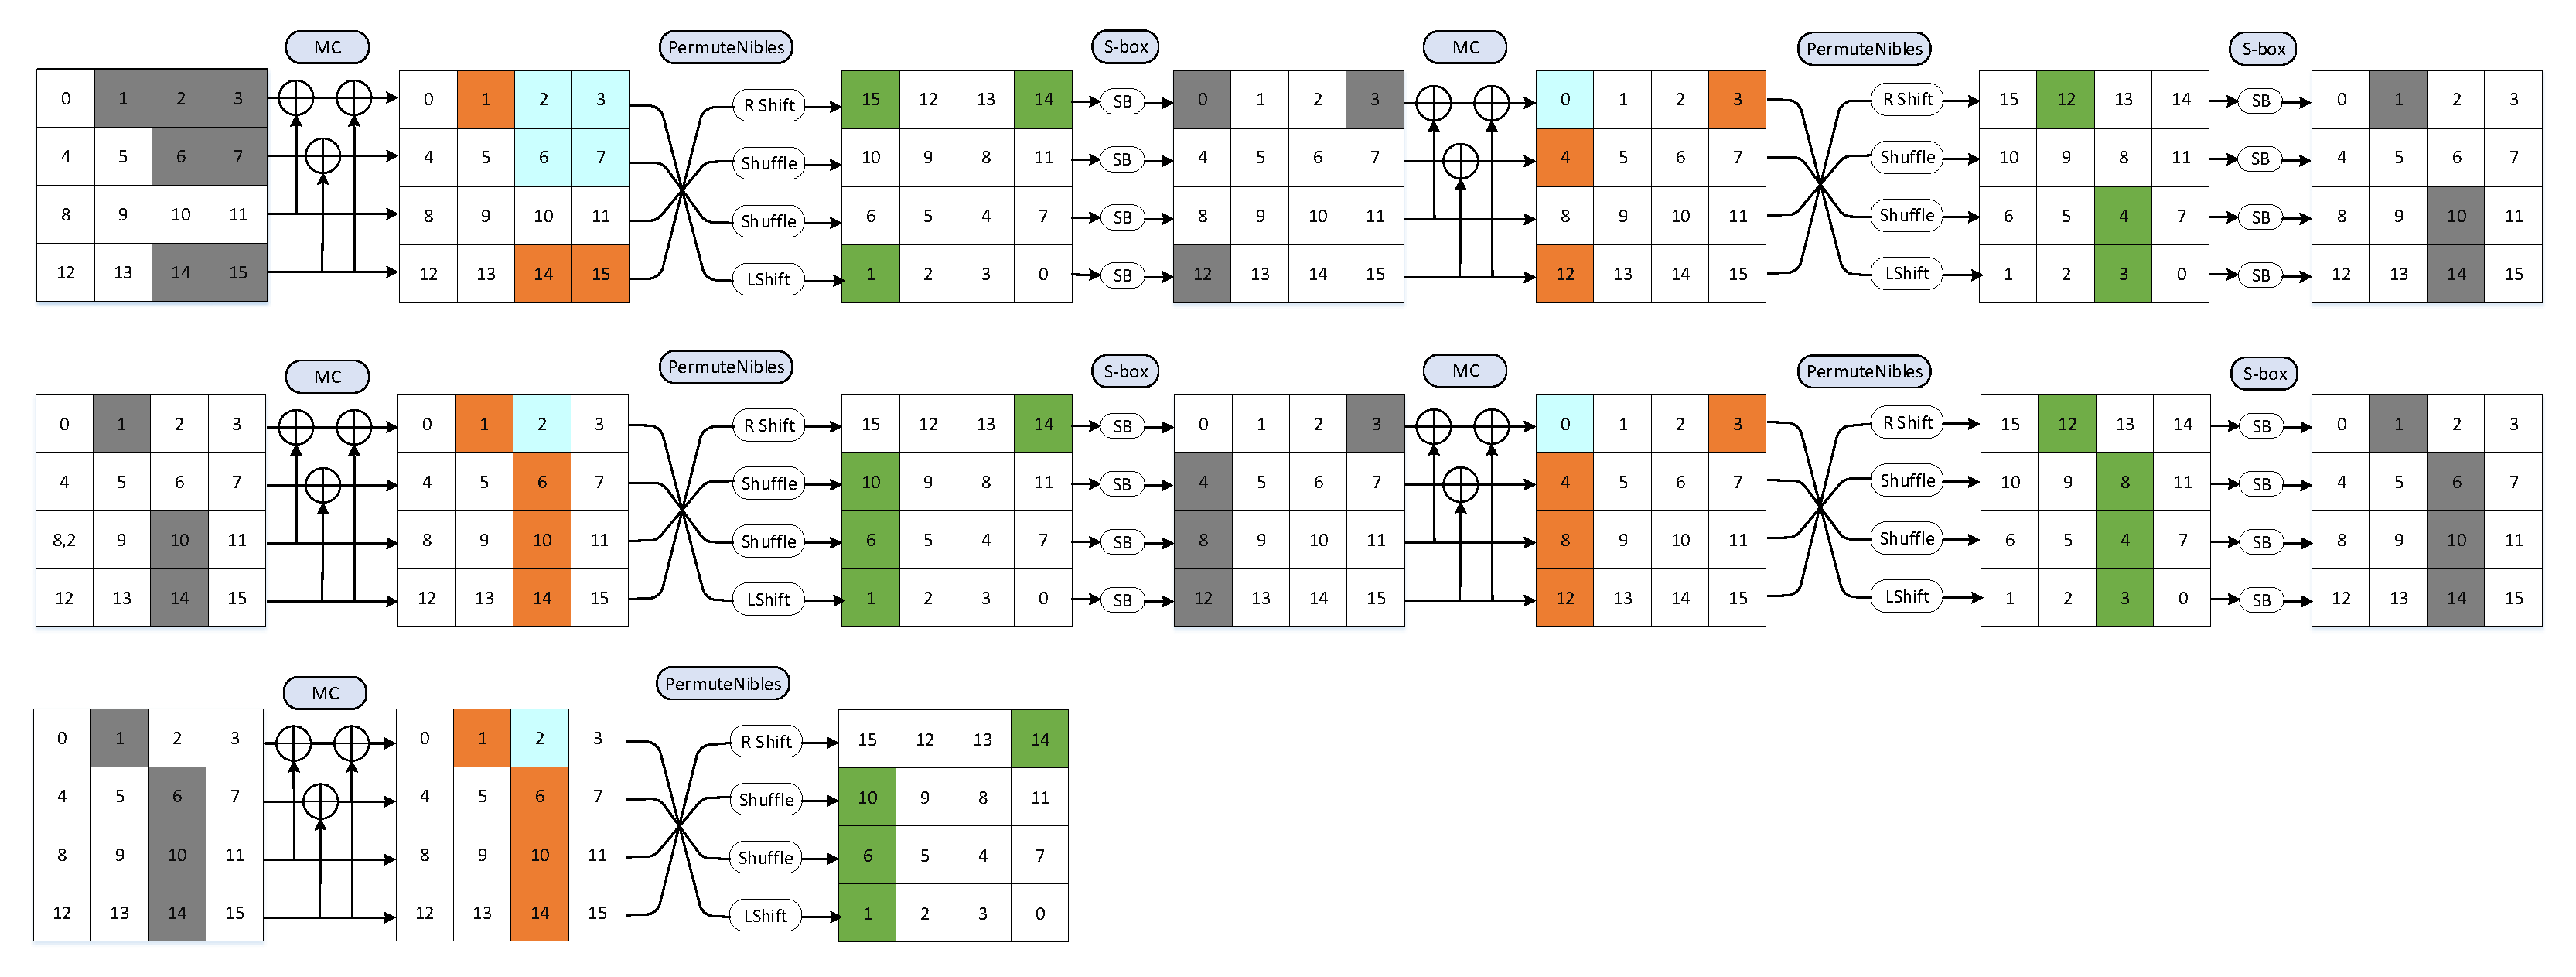
\includegraphics[width=130mm]{./Images/Einevennew.pdf}\\
% $E^{even}_{in,4}$\\\hline
% 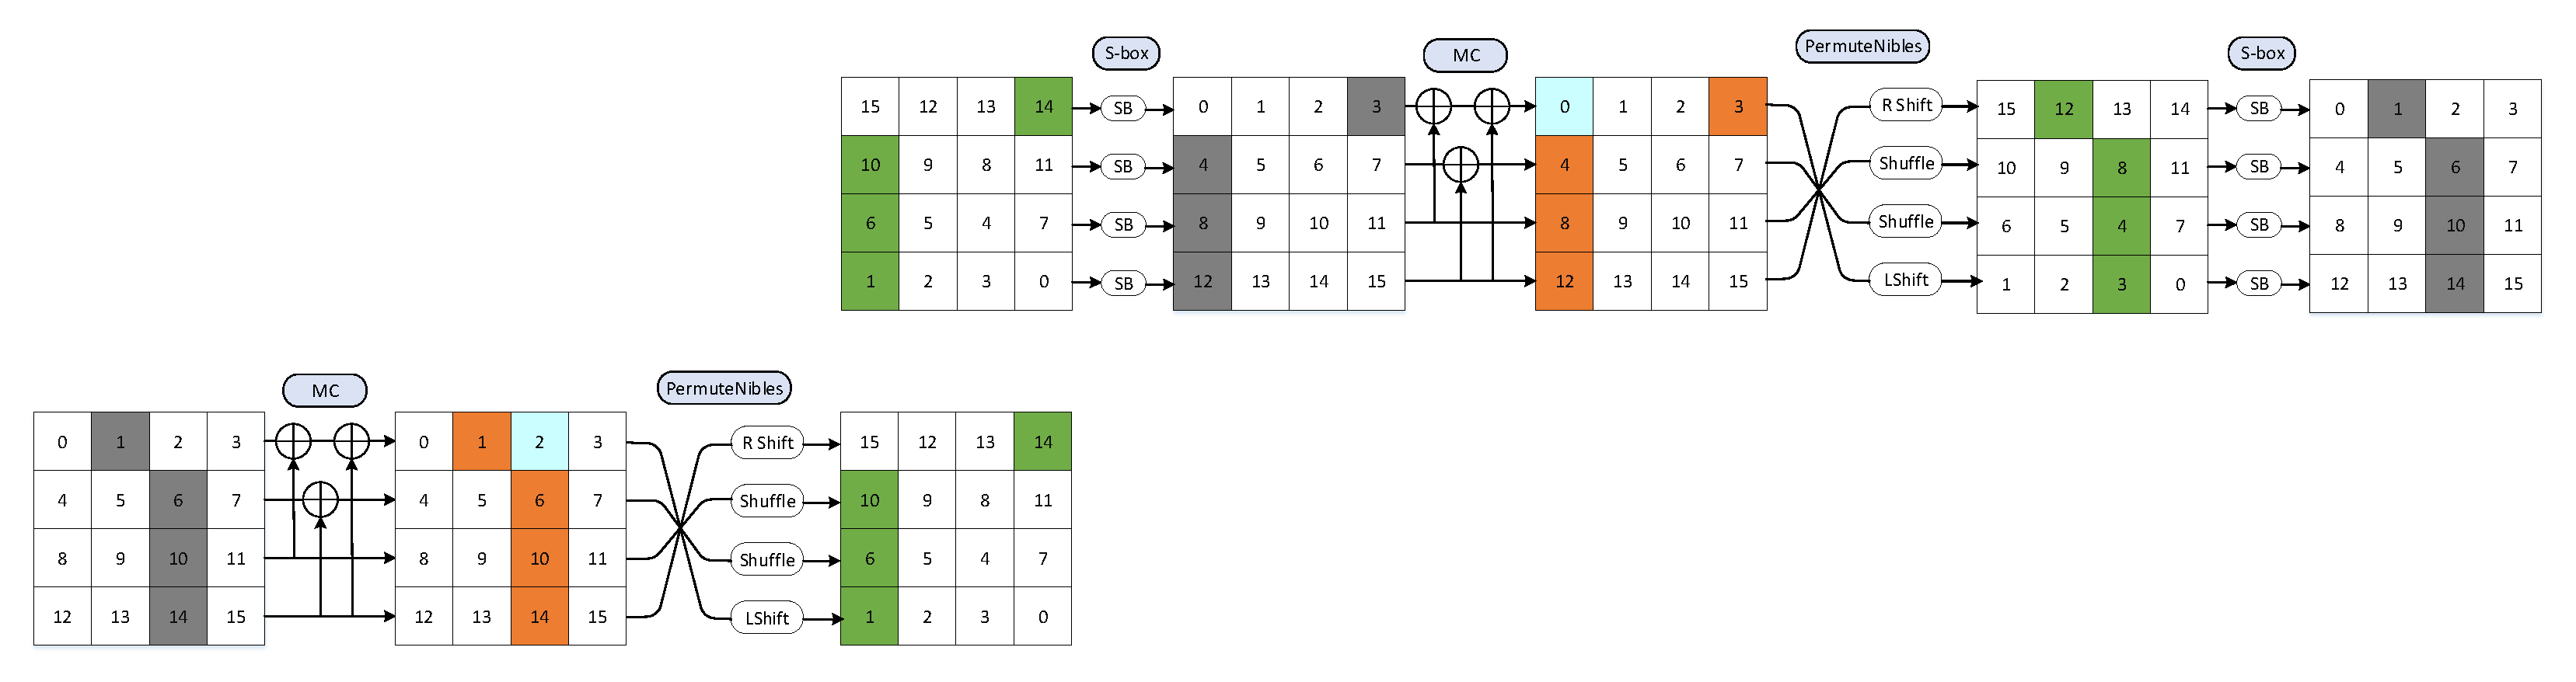
\includegraphics[width=130mm]{./Images/Emevennew}\\
% $E^{even}_{m,2}$\\\hline
% 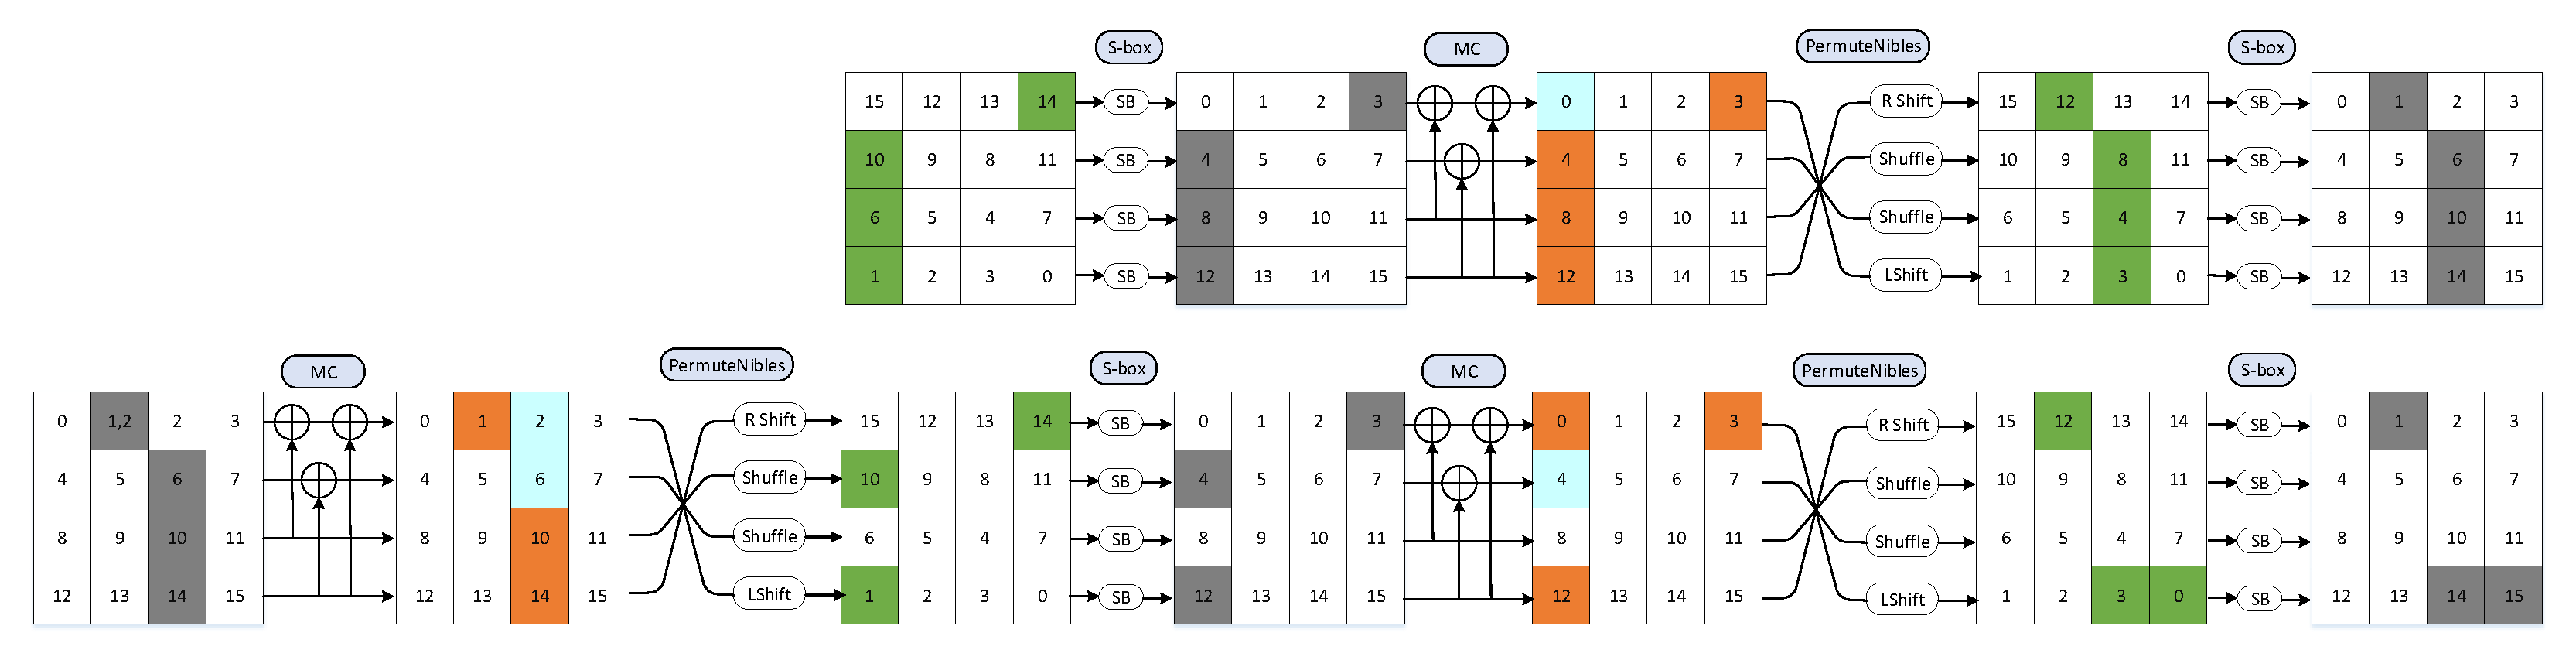
\includegraphics[width=130mm]{./Images/Eoutevennew}\\
% $E^{even}_{out,4}$\\\hline
% \end{tabular}}
% \end{center}
\begin{center}
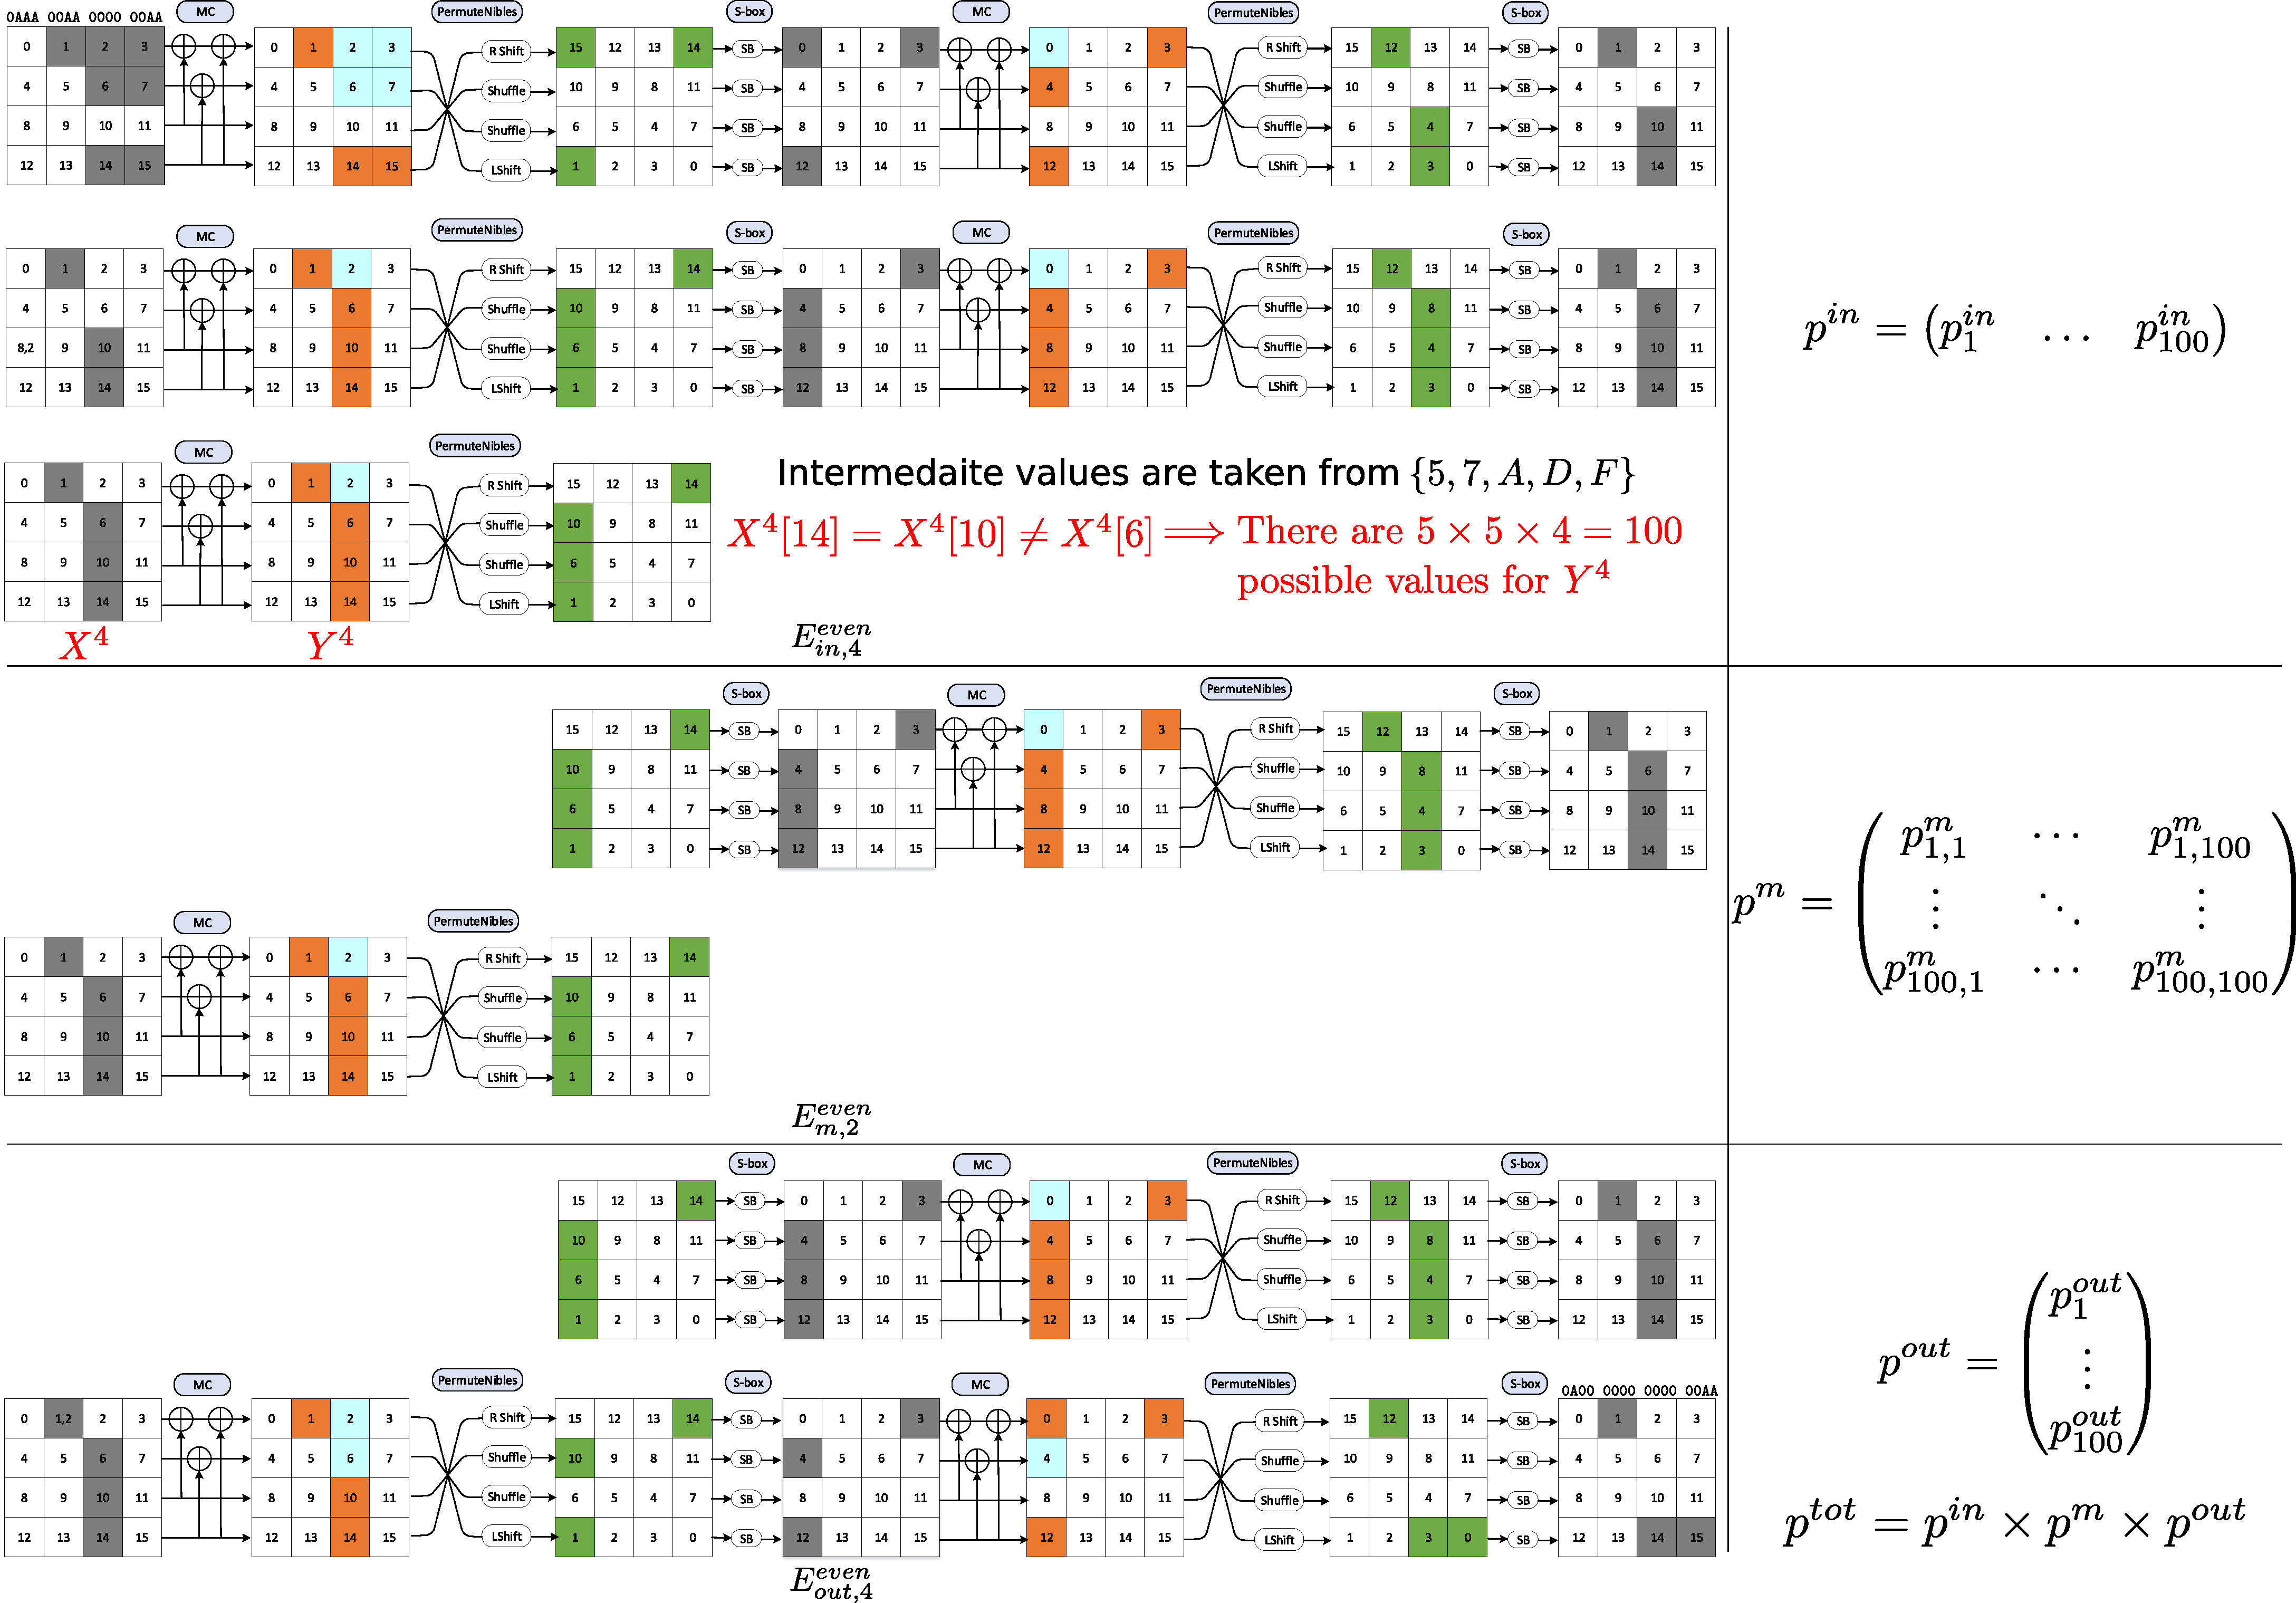
\includegraphics[width=115mm]{./Images/building_blocks_even.pdf}
\end{center}

\end{frame}

% % \begin{frame}{Building Blocks of Odd Number of Rounds}
% % \begin{center}
% % 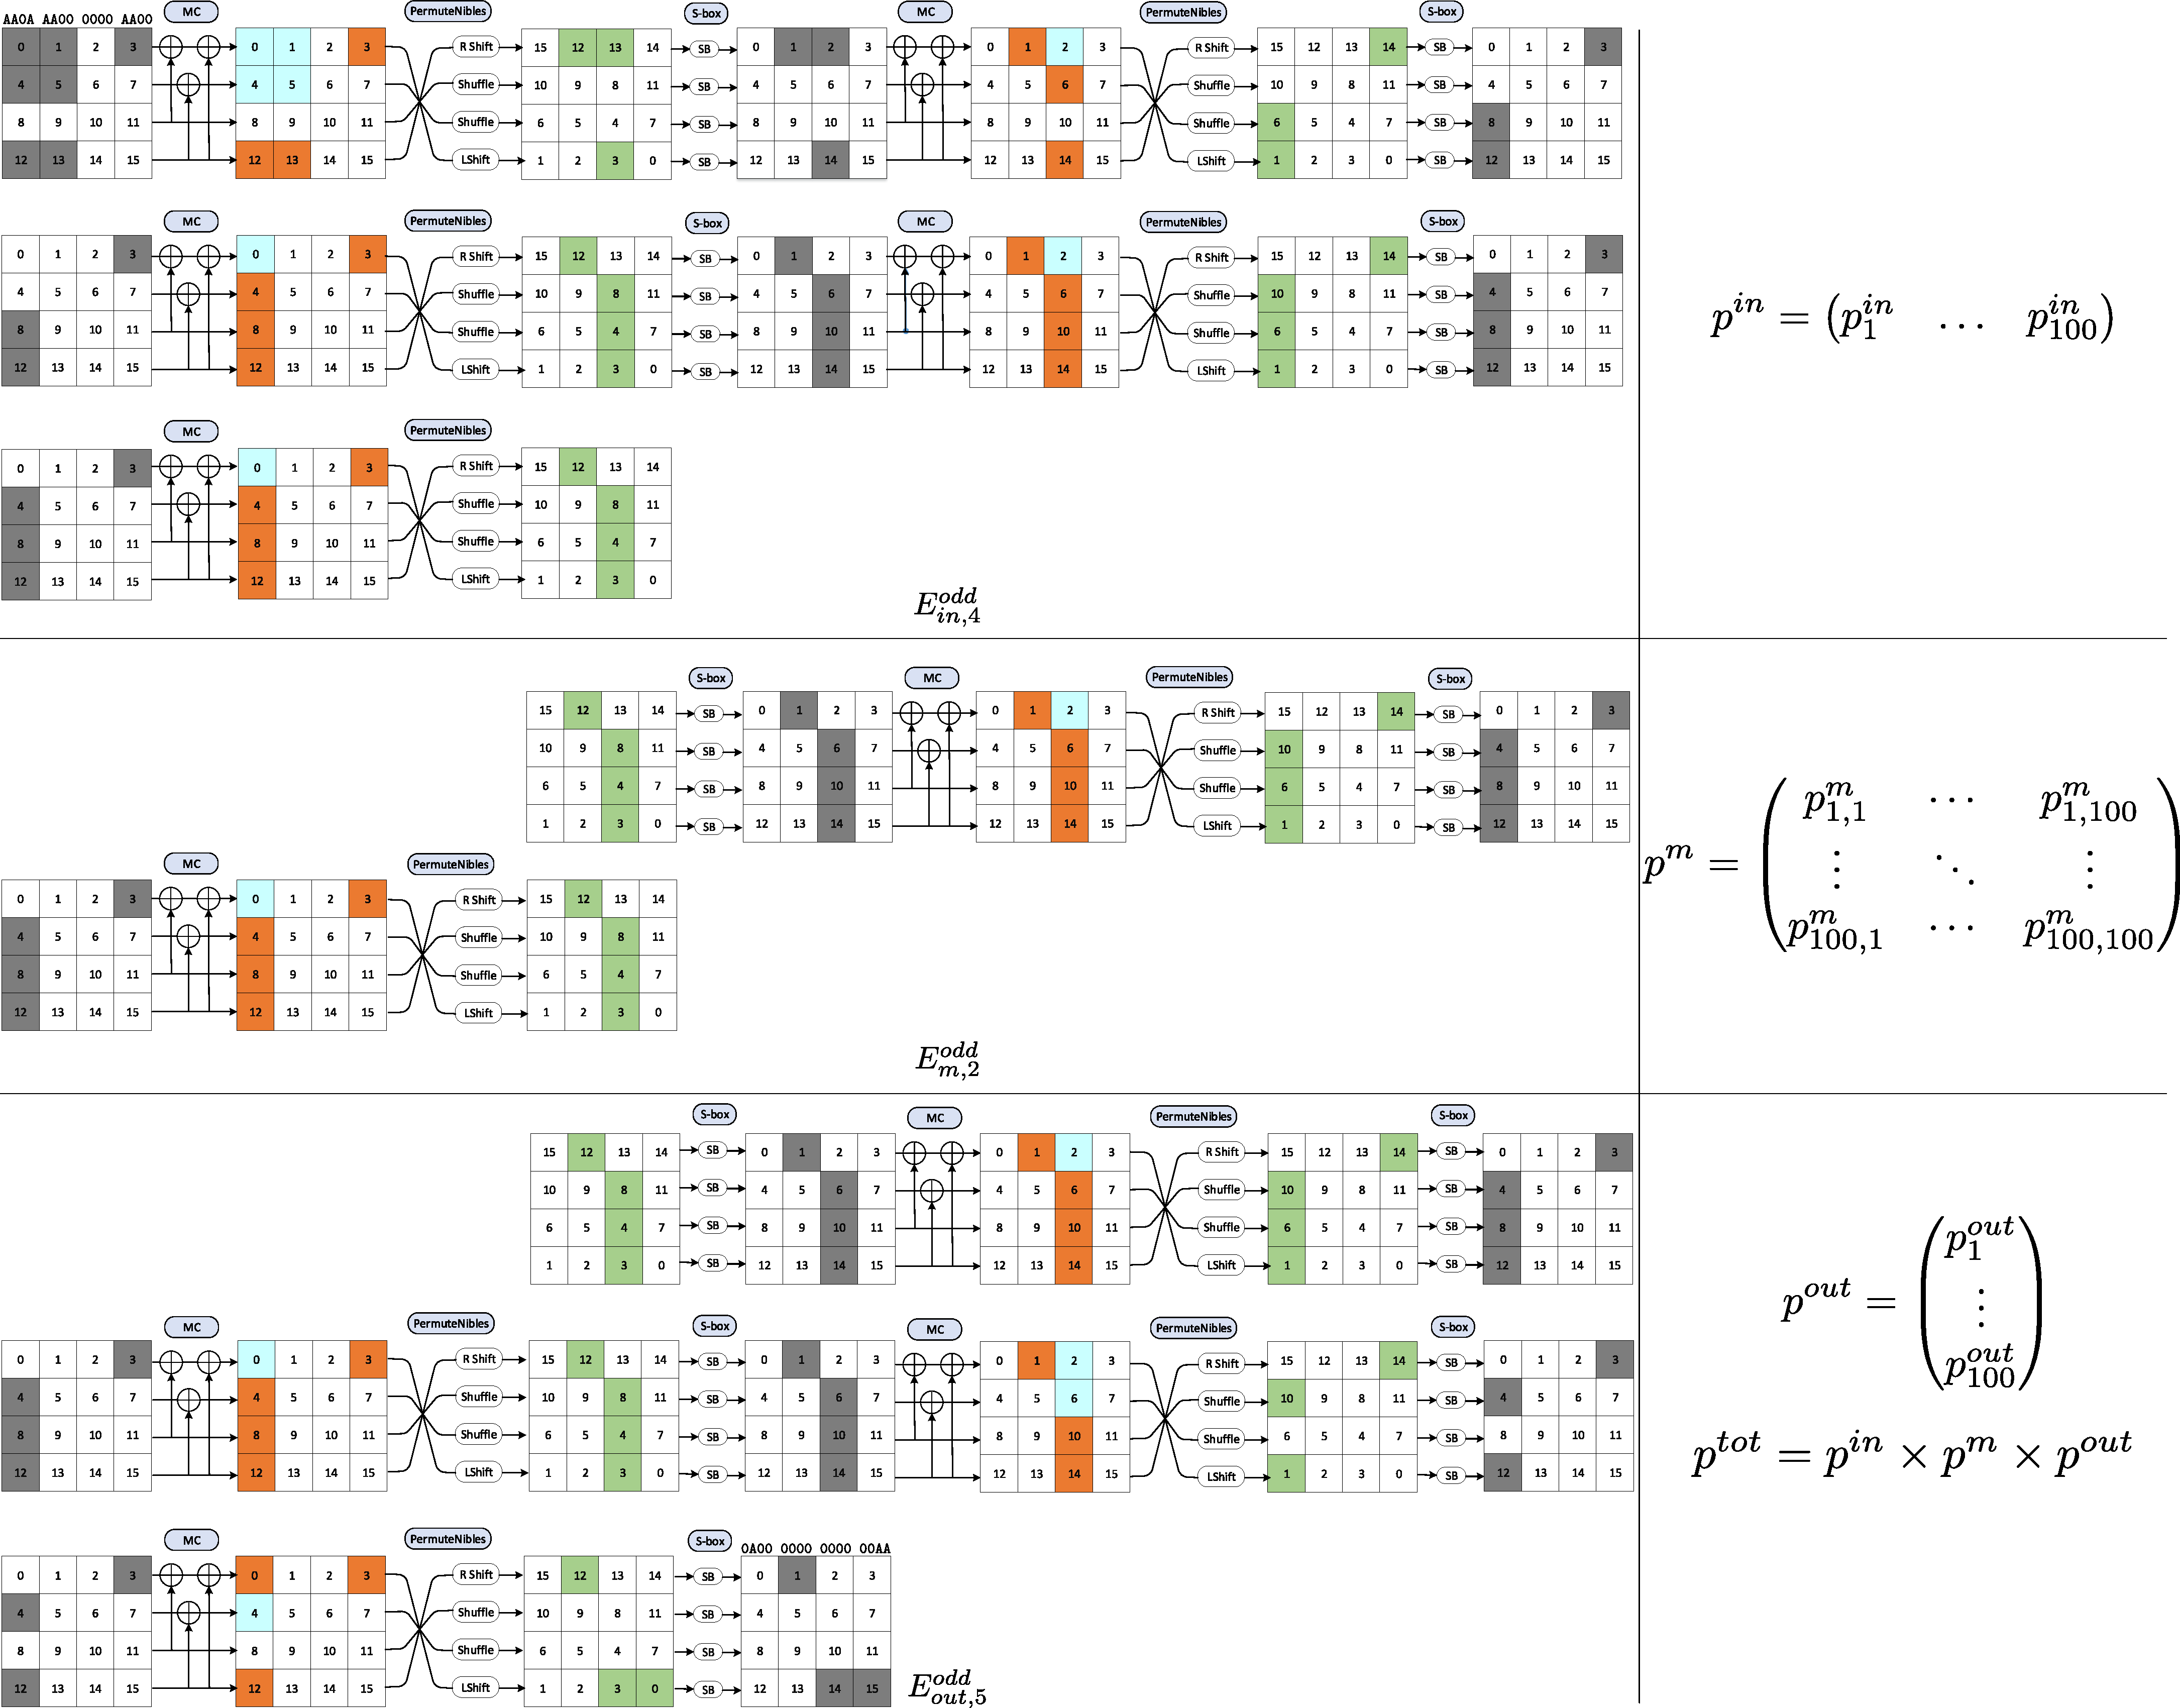
\includegraphics[width=100mm]{./Images/building_blocks_odd.pdf}
% % \end{center}
% % \end{frame}

% % \begin{frame}{Evaluation of Differential Effects}
% % \begin{itemize}
% % \item We used the joint probabilities matrices to determine the differential effect of different round reduced variants of \texttt{CRAFT} 
% % \item In all cases we extended the number of rounds by repeating the middle part ($E^{even/odd}_{m, 2}$) as many times as required:
% % \end{itemize}
% % \begin{center}
% % \scalebox{0.8}{\parbox{.8\linewidth}{
% % \begin{align*}
% % \texttt{AA0A~AA00~0000~AA00} \xrightarrow{\text{9-round; ~$\Pr \geq 2^{-40.20}$}} \texttt{0A00~0000~0000~00AA},\\
% % \texttt{0AAA~00AA~0000~00AA} \xrightarrow{\text{10-round; ~$\Pr \geq 2^{-45.12}$}} \texttt{0A00~0000~0000~00AA},\\
% % \texttt{AA0A~AA00~0000~AA00} \xrightarrow{\text{11-round; ~$\Pr \geq 2^{-49.79}$}} \texttt{0A00~0000~0000~00AA},\\
% % \texttt{0AAA~00AA~0000~00AA} \xrightarrow{\text{12-round; ~$\Pr \geq 2^{-54.72}$}} \texttt{0A00~0000~0000~00AA},\\
% % \texttt{AA0A~AA00~0000~AA00} \xrightarrow{\text{13-round; ~$\Pr \geq 2^{-59.39}$}} \texttt{0A00~0000~0000~00AA},\\
% % \texttt{0AAA~00AA~0000~00AA} \xrightarrow{\text{14-round; ~$\Pr \geq 2^{-64.32}$}} \texttt{0A00~0000~0000~00AA},\\
% % \texttt{AA0A~AA00~0000~AA00} \xrightarrow{\text{15-round; ~$\Pr \geq 2^{-68.99}$}} \texttt{0A00~0000~0000~00AA}.\\
% % \end{align*}
% % }}
% % \end{center}
% % \end{frame}

% % \begin{frame}{Impact of Non-Optimum Trails}
% % \begin{itemize}
% %     \item Since the optimum truncated pattern for a fixed input/output differences is unique, we are able to count the exact number of the optimum trails for any number of rounds of \texttt{CRAFT}, starting from 9, for a given IO differences
% %     \item 
% %     For a fixed IO differences, changing $r_{in}$, $r_{m}$, and $r_{out}$, has an influence on the number of non-optimum trails
% %     \item Improving the previous bounds by considering $r_{m} = 4$, (for even/odd rounds), and $r_{out} = 6$ (for even rounds):
% % \end{itemize}
% % \begin{center}
% % \scalebox{0.8}{\parbox{.8\linewidth}{
% % \begin{align*}
% % \texttt{0AAA~00AA~0000~00AA} \xrightarrow{\text{10-round; ~$\Pr \geq 2^{-44.89}$}} \texttt{0A00~0000~0000~00AA},\\
% %  \texttt{0AAA~00AA~0000~00AA} \xrightarrow{\text{12-round; ~$\Pr \geq 2^{-54.48}$}} \texttt{0A00~0000~0000~00AA},\\
% %  \texttt{AA0A~AA00~0000~AA00} \xrightarrow{\text{13-round; ~$\Pr \geq 2^{-59.13}$}} \texttt{0A00~0000~0000~00AA},\\
% %  \texttt{0AAA~00AA~0000~00AA} \xrightarrow{\text{14-round; ~$\Pr \geq 2^{-63.80}$}} \texttt{0A00~0000~0000~00AA},\\
% %  \texttt{AA0A~AA00~0000~AA00} \xrightarrow{\text{15-round; ~$\Pr \geq 2^{-68.75}$}} \texttt{0A00~0000~0000~00AA}.\\
% % \end{align*}
% % }}
% % \end{center}
% % \end{frame}
\subsection{Improving Differential Distinguishers of \texttt{CRAFT}}
\begin{frame}{Improving Differential Distinguishers of \texttt{CRAFT}}
We could improve the differential distinguishers of \texttt{CRAFT} by four rounds in the single tweak model:
\vspace{5mm}
\begin{center}
\begin{tabular}{|c|ccc|c|c|}
\hline
 $\sharp$ Rounds &  $r_{in}$  &  $r_{m}$ & $r_{out}$ &$\Pr$& $\sharp$ optimum trails\\ 
	 	 \hline
9  &  4  & -  & 5&$2^{-40.20}$&$2^{ 23.32}$\\ 
 10 &  4  & -  & 6&$2^{-44.89}$&$2^{26.49}$\\
 11 &  4  & 2  &5 &$2^{-49.79}$&$2^{29.66}$\\ 
 12 &  4  & 2  & 6&$2^{-54.48}$&$2^{32.83}$\\
 13 &  4  & 4  & 5&$2^{-59.13}$&$2^{36.00}$\\
 14 &  4 & 4  & 6&$2^{-63.80}$ &$2^{39.18}$ \\
\hline
\end{tabular}
\end{center}
\end{frame}

% Contribution page
\begin{frame}[fragile]
\frametitle{Contributions}
\begin{table}[!]
\begin{center}
\resizebox{6cm}{!}{
\begin{tabular}{|c|c|c|c|}
\hline
    Attack&$\sharp$ Rounds & Probability & Reference\\ 

\hline
	 \multirow{6}{*}{$ST$-$D$} & 10 & $2^{-62.61}$ &\cite{Craft}\\ 
	 \cline{2-4}
	   & \cellcolor{yellow}10 & \cellcolor{yellow}$2^{-44.89}$ &\multirow{5}{*}{}\cellcolor{yellow}\\
	   & \cellcolor{yellow}11 & \cellcolor{yellow}$2^{-49.79}$ &\cellcolor{yellow}\\
	   & \cellcolor{yellow}12 & \cellcolor{yellow}$2^{-54.48}$ &\cellcolor{yellow} this paper\\
	   & \cellcolor{yellow}13 & \cellcolor{yellow}$2^{-59.13}$ &\cellcolor{yellow}\\
	   & \cellcolor{yellow}14 & \cellcolor{yellow}$2^{-63.80}$ &\cellcolor{yellow}\\
	 \cline{1-4}
	 $ST$-$TD$ & 12 & $2^{-36}$&\cite{cryptoeprint:2019:126}\\
	 \cline{1-4}
      \hline
	  	  $ST$-$LH$ & 14 & $2^{-62.12}$ &\cite{Craft}\\
	  	  \hline
	% \multirow{6}{*}{$ST$-$LH$} & 14 & $2^{-62.12}$ &\cite{Craft}\\ 
	 %\cline{2-4}
	   %& 9 & $2^{-42.56}$ &\multirow{5}{*}{this paper}\\
	   %& 10 & $2^{-47.12}$ &\\
	   %& 11 & $2^{-52.19}$ &\\
	   %& 12 & $2^{-56.47}$ &\\
	   %& 13 & $2^{-60.96}$ &\\
	 %\cline{1-4}
 %&\multirow{5}{*}{\cite{Craft}}\\
	  %\cline{1-3}
	  $RT_{0}$-$D$ & 15 & $2^{-55.14}$ &\multirow{5}{*}{\cite{Craft}}\\ 
	   $RT_{1}$-$D$ & 16 & $2^{-57.18}$ &\\ 
	   $RT_{2}$-$D$ & 17 & $2^{-60.14}$ &\\
	   $RT_{3}$-$D$ & 16 & $2^{-55.14}$ &\\ 
	   \cline{1-3}
	  $ST$-$ID$ & 13 & - &\\ 
	  \cline{1-3}
	  $ST$-$INT$ & 13 & - &\\ 
	   \cline{1-3}
	  	 $ST$-$ZC$ & 13 & - &\\ 
	  	 \hline
	  	 $RT$-$ZC$ & \cellcolor{yellow} 14 & \cellcolor{yellow}- & \cellcolor{yellow}this paper\\
	  \hline
	  	  $RT$-$INT$ & \cellcolor{yellow} 14 & \cellcolor{yellow}- &\cellcolor{yellow}this paper\\
	  \hline
	   $RK$-$D$ & 32 & $2^{-32}$ &\cite{Amr}\\
	  \hline
	\end{tabular}
	}
	\label{Summary_attacks_table}
\end{center}
\end{table}
\end{frame}

\begin{frame}
\Huge{\centerline{Thank You for Listening!}}
\begin{center}
\small{all the codes are publicly available via the following link:

% 
\includegraphics[scale=0.05]{./Images/hadipourh.jpeg}

\href{https://github.com/hadipourh/craftanalysis}{https://github.com/hadipourh/craftanalysis}}    
\end{center}
\end{frame}

\begin{frame}[allowframebreaks, fragile]{Bibliography}
\bibliographystyle{plain}
\bibliography{biblio.bib}
\end{frame}

% \begin{frame}{\TeX{}}
% 	\begin{columns}
% 		\begin{column}{4cm}
% 			\begin{figure}
%   				\includegraphics[height=3cm]{384px-KnuthAtOpenContentAlliance.jpg}
%   				\includegraphics[height=3cm]{ArtOfComputerProgramming.jpg}
% 			\end{figure}
% 			\begin{center}
% 				\tiny
% 				Donald Knuth \\
% 				Computer Scientist \\
% 				Born January 10, 1938 (age 77) \\
% 			\end{center}
% 		\end{column}
% 		\begin{column}{6cm}
% 			\begin{itemize}
% 				\item \TeX{} was created by Donald Knuth in 1978
% 				\pause
% 				\item A typesetting macro language and compiler:
% 				\begin{itemize}
% 					\item Readable mathematics
% 					\item Better hyphenation
% 					\item Optimized justification
% 					\item Font management tools
% 					\item Cross-compatibility
% 				\end{itemize}
% 				\pause
% 				\item Code -- Compile -- Visualize
% 			\end{itemize}
% 		\end{column}
% 	\end{columns}
% \end{frame}

% \begin{frame}{\LaTeX{}}
% \begin{columns}
% \begin{column}{4cm}
% \begin{figure}
%   \includegraphics[height=3cm]{leslie.jpg}
%   \includegraphics[height=3cm]{latex.jpg}
% \end{figure}
% \begin{center}
% \tiny
% Leslie Lamport \\
% Computer Scientist \\
% Born February 7, 1941 (age 74) \\
% \end{center}
% \end{column}
% \begin{column}{6cm}
% \begin{itemize}
% \item \LaTeX{} $=$ Leslie Lamport's \TeX{}
% \pause
% \item Initial Release in 1984
% \pause
% \item A macro package for \TeX{} with:
% \begin{itemize}
% \item Document Types
% \item Chapter Headings
% \item Footnotes
% \item Cross-references
% \item Bibliographies
% \item Environments (Tables, Figures, Equations)
% \end{itemize}
% \end{itemize}
% \end{column}
% \end{columns}
% \end{frame}

% \subsection{Tables and Figures}

% \begin{frame}{Tables and Figures}

% \begin{itemize}
% \item Use \texttt{tabular} for basic tables --- see Table~\ref{tab:widgets}, for example.
% \item You can upload a figure (JPEG, PNG or PDF) using the files menu. 
% \item To include it in your document, use the \texttt{includegraphics} command (see the comment below in the source code).
% \end{itemize}

% Commands to include a figure:
%\begin{figure}
%\includegraphics[width=\textwidth]{your-figure's-file-name}
%\caption{\label{fig:your-figure}Caption goes here.}
%\end{figure}

% \begin{table}
% \centering
% \begin{tabular}{l|r}
% Item & Quantity \\\hline
% Widgets & 42 \\
% Gadgets & 13
% \end{tabular}
% \caption{\label{tab:widgets}An example table.}
% \end{table}

% \end{frame}

% \subsection{Mathematics}

% \begin{frame}{Readable Mathematics}

% Let $X_1, X_2, \ldots, X_n$ be a sequence of independent and identically distributed random variables with $\text{E}[X_i] = \mu$ and $\text{Var}[X_i] = \sigma^2 < \infty$, and let
% $$S_n = \frac{X_1 + X_2 + \cdots + X_n}{n}
%       = \frac{1}{n}\sum_{i}^{n} X_i$$
% denote their mean. Then as $n$ approaches infinity, the random variables $\sqrt{n}(S_n - \mu)$ converge in distribution to a normal $\mathcal{N}(0, \sigma^2)$.

% \end{frame}

% \begin{frame}{Editors and Compilers}
% \begin{itemize}
% \item To install in your machine
% \begin{itemize}
% \item Check \texttt{latex-project.org}
% \end{itemize}
% \pause
% \item In the cloud
% \begin{itemize}
% \item ShareLatex : \texttt{www.sharelatex.com}
% \item Overleaf : \texttt{www.overleaf.com}
% \end{itemize}
% \end{itemize}
% \pause
% \vskip 1cm
% \begin{block}{Please give me Mb of space on Overleaf}
% https://www.overleaf.com/signup?ref=d1806010dac8
% \end{block}
% \end{frame}

% \begin{frame}[fragile]{Hello \LaTeX{} World!}
% \begin{columns}
% \begin{column}{5cm}
% \vspace{-2cm}
% \lstinputlisting{file1.tex}
% \end{column}
% \begin{column}{5cm}
% Hello \LaTeX{} World!
% \end{column}
% \end{columns}
% \end{frame}

% \begin{frame}[fragile]{More structure}
% \begin{columns}
% \begin{column}{5.5cm}
% \lstinputlisting[basicstyle=\sffamily\tiny,]{file2.tex}
% \end{column}
% \begin{column}{4.5cm}
% \vspace{-2cm}
% \begin{figure}
% \includegraphics[width=6cm]{file2a.pdf}
% \end{figure}
% \end{column}
% \end{columns}
% \end{frame}

% \begin{frame}[fragile]{Team work}
% \begin{columns}
% \begin{column}{5cm}
% \lstinputlisting[basicstyle=\sffamily\tiny,]{file3.tex}
% \end{column}
% \begin{column}{5cm}
% \begin{itemize}
% \item Using the \texttt{include} macro, each author can work on an independent file. 
% \item To compile only a set of files, use the macro \texttt{includeonly}
% \item Welcome to team work in \LaTeX{}!
% \end{itemize}
% \end{column}
% \end{columns}
% \end{frame}

%\begin{frame}{LaTeX{} Basics}
% 		\begin{itemize}
%         	\item Documents
%         	\item Fonts and Styles
%             \item Text Symbols
%             \item Paragraphs
%             \item Lists
%             \item Cross References
%             \item Tables
%             \item Math Symbols
%         	\item Equations
%             \item Figures
%             \item Bibliography
% 		\end{itemize}
% 	\end{frame}

%\begin{frame}{Documents}
%     	\begin{columns}
%         	\begin{column}{3cm}
%               Classes:
%               \begin{itemize}
%                   \item \texttt{book}
%                   \item \texttt{article}
%                   \item \texttt{report}
%                   \item \texttt{letter}
%                   \item \texttt{slides}
%                   \item \texttt{beamer}
%                   \item \texttt{IEEETran}
%                   \item \texttt{minimal}
%                   \item \ldots
%               \end{itemize}
%         	\end{column}
%             \begin{column}{7cm}
%               Options:
%               \begin{itemize}
%                   \item \texttt{10pt, 11pt, 12pt}
%                   \item \texttt{a4paper, letterpaper,\ldots}
%                   \item \texttt{fleqn, leqno}
%                   \item \texttt{titlepage, notitlepage}
%                   \item \texttt{twocolumn}
%                   \item \texttt{twoside, oneside}
%                   \item \texttt{landscape}
%                   \item \texttt{openright, openany}
%                   \item \texttt{draft}
%               \end{itemize}
%         	\end{column}
%     	\end{columns}
% 	\end{frame}

%\begin{frame}[fragile]
% \frametitle{Fonts and Styles}
% \begin{tabular}[c]{|l l|l l|}
% \hline
% \verb!\textrm{Hello}! & \textrm{Hello} & \verb!{\tiny Hello}! & {\tiny Hello} \\
% \hline
% \verb!\textsf{Hello}! & \textsf{Hello} & \verb!{\scriptsize Hello}! & {\scriptsize Hello} \\
% \hline
% \verb!\texttt{Hello}! & \texttt{Hello} & \verb!{\footnotesize Hello}! & {\footnotesize Hello} \\
% \hline
% \verb!\textmd{Hello}! & \textmd{Hello} & \verb!{\small Hello}! & {\small Hello} \\
% \hline
% \verb!\textbf{Hello}! & \textbf{Hello} & \verb!{\normalsize Hello}! & {\normalsize Hello} \\
% \hline
% \verb!\textup{Hello}! & \textup{Hello} & \verb!{\large Hello}! & {\large Hello} \\
% \hline
% \verb!\textit{Hello}! & \textit{Hello} & \verb!{\Large Hello}! & {\Large Hello} \\
% \hline
% \verb!\textsl{Hello}! & \textsl{Hello} & \verb!{\LARGE Hello}! & {\LARGE Hello} \\
% \hline
% \verb!\underline{Hello}! & \underline{Hello} & \verb!{\huge Hello}! & {\huge Hello} \\
% \hline
% \verb!\textsc{Hello}! & \textsc{Hello} & \verb!{\Huge Hello}! & {\Huge Hello} \\
% \hline
% \end{tabular}
% \end{frame}
        
%\begin{frame}[fragile]
% \frametitle{Text Symbols}
% \begin{center}
% \begin{tabular}[c]{|l l|l l|l l|}
% \hline
% \verb!\$! & \$ & \verb!``! & ``  & \verb!\oe! & \oe \\
% \hline
% \verb!\&! & \& & \verb!''! & '' & \verb!\OE! & \OE\\
% \hline
% \verb!\%! & \% & \verb!"! & " & \verb!\ae! & \ae\\
% \hline
% \verb!\#! & \# & \verb!\'a! & \'a & \verb!\AE! & \AE\\
% \hline
% \verb!\S! & \S & \verb!\`a! & \`a & \verb!\o! & \o\\
% \hline
% \verb!\LaTeX{}! & \LaTeX{} & \verb!\~a! & \~a & \verb!\O! & \O\\
% \hline
% \verb!A\_B! & A\_B & \verb!\^a! & \^a & \verb!\l! & \l\\
% \hline
% \verb!\textbar! & \textbar & \verb!\c a! & \c a & \verb!\L! & \L\\
% \hline
% \verb!\textbullet! & \textbullet & \verb!\"a! & \"a & \verb!\i! & \i\\
% \hline
% \verb!\textbackslash! & \textbackslash & \verb!\v a! & \v a & \verb!\j! & \j\\
% \hline
% \verb!\ldots! & \ldots & \verb!\H a! & \H a & \verb!\aa! & \aa\\
% \hline
% \verb!\~{}! &\~{} & \verb!\=a! & \=a & \verb!\AA! & \AA\\
% \hline
% \verb!\^{}! &\^{} & \verb!\d a! & \d a & \verb!A-B! & A-B\\
% \hline
% \verb!\textless! & \textless & \verb!\.a! & \.a & \verb!A--B! & A--B\\
% \hline
% \verb!\textgreater! & \textgreater & \verb!\b a! & \b a & \verb!A---B! & A---B\\
% \hline
% \end{tabular} 
% \end{center}
% \end{frame}

%\begin{frame}[fragile]{Paragraphs}
% \begin{columns}
% \begin{column}{6cm}
% \vspace{-0.3cm}
% \begin{lstlisting}
% \begin{center}
% Please give me space on Overleaf
% \end{center}
% \end{lstlisting}
% \begin{lstlisting}
% \begin{flushleft}
% Please give me space on Overleaf
% \end{flushleft}
% \end{lstlisting}
% \begin{lstlisting}
% \begin{flushright}
% Please give me space on Overleaf
% \end{flushright}
% \end{lstlisting}
% \begin{lstlisting}
% \begin{quote}
% Please give me space on Overleaf
% \end{quote}
% \end{lstlisting}
% \begin{lstlisting}
% \begin{quotation}
% Please give me space on Overleaf
% \end{quotation}
% \end{lstlisting}
% \begin{lstlisting}
% \begin{verse}
% Please give me space on Overleaf
% \end{verse}
% \end{lstlisting}
% \end{column}
% \begin{column}{4cm}
% \vspace{-0.5cm}
% \footnotesize
% \begin{center}
% Please give me space on Overleaf
% \end{center}
% \begin{flushleft}
% Please give me space on Overleaf
% \end{flushleft}
% \begin{flushright}
% Please give me space on Overleaf
% \end{flushright}
% \begin{quote}
% Please give me space on Overleaf
% \end{quote}
% \begin{quotation}
% Please give me space on Overleaf
% \end{quotation}
% \begin{verse}
% Please give me space on Overleaf
% \end{verse}
% \end{column}
% \end{columns}
% \end{frame}

%\begin{frame}[fragile]{Paragraphs}
% \begin{columns}
% \begin{column}{6cm}
% \vspace{-0.3cm}
% \begin{lstlisting}
% \begin{itemize}
% \item One item
% \item Another item
% \end{itemize}
% \end{lstlisting}
% \begin{lstlisting}
% \begin{enumerate}
% \item First item
% \item Second item
% \end{enumerate}
% \end{lstlisting}
% \begin{lstlisting}
% \begin{description}
% \item[Lion] A mammal
% \item[Shark] A fish
% \end{description}
% \end{lstlisting}
% \begin{lstlisting}
% \begin{itemize}
% \item A list inside a list
% \begin{enumerate}
% \item Lists 
% \item can be 
% \item recursive
% \end{enumerate}
% \end{itemize}
% \end{lstlisting}
% \end{column}
% \begin{column}{4cm}
% \vspace{-1cm}
% \footnotesize
% \begin{itemize}
% \item One item
% \item Another item
% \end{itemize}
% \vspace{0.5cm}
% \begin{enumerate}
% \item First item
% \item Second item
% \end{enumerate}
% \vspace{0.5cm}
% \begin{description}
% \item[Lion] A mammal
% \item[Shark] A fish
% \end{description}
% \vspace{0.5cm}
% \begin{itemize}
% \item A list inside a list
% \begin{enumerate}
% \item Lists 
% \item can be 
% \item recursive
% \end{enumerate}
% \end{itemize}
% \end{column}
% \end{columns}
% \end{frame}

%\begin{frame}[fragile]{Cross References}
% \begin{columns}
% \begin{column}{6cm}
% \begin{itemize}
% % \item Numbered items and pages can be referenced anywhere in the text.
% % \item Numbered items can be document elements (parts, chapters, sections, subsections), equations, figures, tables, \ldots
% \item Use macro \verb!\label{!\textit{some-- identifier}\verb!}! to set a mark.
% \item Use macro \verb!\ref{!\textit{some-- identifier}\verb!}! to retrieve the number of the item where the mark is defined.
% \item Use macro \verb!\pageref{!\textit{some-- identifier}\verb!}! to retrieve the page number where mark is defined.
% \end{itemize}
% \begin{lstlisting}
% \label{marcador}
% This is slide \ref{marcador}. \\
% It is in page \pageref{marcador}.
% \end{lstlisting}
% \end{column}
% \begin{column}{4cm}
% \label{marcador}
% \begin{center}
% This is slide \ref{marcador}. \\
% It is in page \pageref{marcador}.
% \end{center}
% \end{column}
% \end{columns}
% \end{frame}

%\begin{frame}[fragile]{Tables}
% \begin{lstlisting}
% \begin{table}
% \begin{tabular}{ l | c | r | p{6cm}}
% Name & Age & Height & Email \\
% \hline
% Alex & 44 & 1,80m & alex@isr.ist.utl.pt \\
% \end{tabular}
% \caption{JEEC 2015 Monday Workshop Participants}
% \end{table}
% \end{lstlisting}
% \begin{table}
% \begin{tabular}{ l | c | r | p{6cm}}
% Name & Age & Height & Email \\
% \hline
% Alex & 44 & 1,80m & alex@isr.ist.utl.pt \\
% \end{tabular}
% \caption{JEEC 2015 Monday Workshop Participants}
% \end{table}
% \end{frame}

%\begin{frame}[fragile]{Math Symbols}
% \begin{columns}
% \begin{column}{4.5cm}
% \begin{lstlisting}
% Equation $E_c=\frac{mv^2}{2}$ is true
% \end{lstlisting}

% \begin{block}{}
% Equation $E_c=\frac{mv^2}{2}$ is true
% \end{block}
% \vspace{0.5cm}
% \begin{lstlisting}
% Equation \[E_c=\frac{mv^2}{2}\] is true
% \end{lstlisting}

% \begin{block}{}
% Equation \[E_c=\frac{mv^2}{2}\] is true
% \end{block}
% \end{column}
% \begin{column}{5.5cm}
% \begin{center}
% \scriptsize
% \begin{tabular}{| l l | l l|}
% \hline
% \verb!\sqrt[n]{x}! & $\sqrt[n]{x}$ & \verb!\alpha! & $\alpha$
% \\
% \hline
% \verb!\sum_{k=1}^N! & $\sum_{k=1}^N$ & \verb!\beta! & $\beta$
% \\
% \hline
% \verb!\int_{k=1}^N! & $\int_{k=1}^N$ & \verb!\leq! & $\leq$
% \\
% \hline
% \verb!\prod_{k=1}^N! & $\prod_{k=1}^N$ & \verb!\geq! & $\geq$
% \\
% \hline
% \verb!\overbrace{ab}! & $\overbrace{ab}$ & \verb!\infty! & $\infty$
% \\
% \hline
% \verb!\widetilde{ab}! & $\widetilde{ab}$ & \verb!\times! & $\times$
% \\
% \hline
% \verb!\Rightarrow! & $\Rightarrow$ & \verb!\forall! & $\forall$
% \\
% \hline
% \verb!\Updownarrow! & $\Updownarrow$ & \verb!\exists! & $\exists$
% \\
% \hline
% \verb!\tilde{a}! & $\tilde{a}$ & \verb!\in! & $\in$
% \\
% \hline
% \verb!\hat{a}! & $\hat{a}$ & \verb!\pm! & $\pm$
% \\
% \hline
% \verb!\dot{a}! & $\dot{a}$ & \verb!\neq! & $\neq$ \\
% \hline
% \verb!\ddot{a}! & $\ddot{a}$ & \verb!\mid! & $\mid$
% \\
% \hline
% \verb!\arctan! & $\arctan$ & \verb!\subset! & $\subset$
% \\
% \hline
% \verb!\limsup! & $\limsup$ & \verb!\cup! & $\cup$
% \\
% \hline
% \verb!\bigotimes! & $\bigotimes$ & \verb!\angle! & $\angle$
% \\
% \hline
% \verb!\bigodot! & $\bigodot$ & \verb!\cdots! & $\cdots$
% \\
% \hline
% \verb!\approx! & $\approx$ & \verb!\flat! & $\flat$
% \\
% \hline
% \verb!\doteq! & $\doteq$ & \verb!\Box! & $\Box$
% \\
% \hline
% \verb!\emptyset! & $\emptyset$ & \verb!\partial! & $\partial$
% \\
% \hline
% \end{tabular}
% \end{center}
% \end{column}
% \end{columns}
% \end{frame}

%\begin{frame}[fragile]{Equations}
% The \texttt{equation} environment automatically numbers equations. 

% If numbering is not needed use \texttt{equation*}.
% \begin{lstlisting}
% \begin{equation}
% \label{eq:matrix_transpose}
% \left[\begin{array}{ccc} a_{11} & \cdots & a_{1n} \\
% \vdots & \ddots & \vdots \\ a_{n1} & \cdots & a_{nn}
% \end{array}\right]^T= 
% \left[\begin{array}{ccc} a_{11} & \cdots & a_{n1} \\
% \vdots & \ddots & \vdots \\ a_{1n} & \cdots & a_{nn}
% \end{array}\right]
% \end{equation}
% \end{lstlisting}

% \begin{equation}
% \label{eq:matrix_transpose}
% \left[
% \begin{array}{ccc}
% a_{11} & \cdots & a_{1n} \\
% \vdots & \ddots & \vdots \\
% a_{n1} & \cdots & a_{nn}
% \end{array}
% \right]^T
% = 
% \left[
% \begin{array}{ccc}
% a_{11} & \cdots & a_{n1} \\
% \vdots & \ddots & \vdots \\
% a_{1n} & \cdots & a_{nn}
% \end{array}
% \right]
% \end{equation}
% \end{frame}

% \begin{frame}[fragile]{Figures}
% Graphics files (*.jpg, *.png, *.pdf, etc) can be displayed in a \texttt{figure} environment, using command \verb!\includegraphics! from the \texttt{graphicx} package.
% \begin{columns}
% \begin{column}{5cm}
% \begin{lstlisting}
% \usepackage{graphicx}
% \begin{figure}[!htpb]
% \label{fig:leslie}
% \includegraphics[width=2.5cm]{leslie.jpg}
% \includegraphics[width=2.5cm]{texbook.jpg}
% \caption{Leslie Lamport and his TeXbook.}
% \end{figure}
% \end{lstlisting}
% \end{column}
% \begin{column}{5cm}
% \begin{figure}[!htpb]
% \label{fig:leslie}
% \includegraphics[width=2.5cm]{leslie.jpg}
% \includegraphics[width=2.5cm]{texbook.jpg}
% \caption{Leslie Lamport and his textbook.}
% \end{figure}
% \end{column}
% \end{columns}
% \end{frame}

% \begin{frame}{Conclusion}
% 		\begin{columns}
% 			\begin{column}{5cm}
% 				\begin{figure}
%   					\includegraphics[height=4cm]{384px-KnuthAtOpenContentAlliance.jpg}
% 				\end{figure}
% 			\end{column}
% 			\begin{column}{5cm}
% 				\begin{flushright}
% 					\textit{The ideal situation occurs when
% the things that we regard as beautiful
% are also regarded by other
% people as useful.}
% 					\vskip 0.5cm
% 				-- Donald Knuth
% 				\end{flushright}
% 			\end{column}
% 		\end{columns}
% 	\end{frame}

\end{document}
